\documentclass[bsc,frontabs,singlespacing,twoside,parskip,deptreport]{infthesis}
%twoside
% Used packages
\usepackage{graphicx}
\usepackage{float}
\usepackage{minted}
\usepackage{hyperref}
\usepackage{caption}
\usepackage{subcaption}
\usepackage{lscape}
\usepackage{blindtext}

\begin{document}
% title{\vspace{-5.0cm} \centering{\includegraphics[scale=1]{path/to/image/file.png}} \\ Automated Source Code Rejuvenation}
\title{\vspace{-5.0cm} Automated Source Code Rejuvenation \\ \vspace{1cm} \centering{
\includegraphics[scale=0.75]{images/shield-crest-UoE.png}} }

\author{Andrew Lindsay}

\course{Master of Informatics}
\project{{\bf MInf Project (Part 1) Report}}

\date{\today}

\abstract{
    
}

\maketitle

\section*{Acknowledgements}
Acknowledgements go here. 

\tableofcontents

%\pagenumbering{arabic}

\chapter{Introduction} \label{Introduction}

% overview

% \section{What is source code rejuvenation ?}

%  add metric about amount of legacy code (hard to find)
Developers throughout their careers will be faced with situations where they inherit or have to work on code they did not write, and which has not been actively developed for some time. This code could be many years old but still, require maintaining as it is part of a larger system within a company. This is a common occurrence within the industry, and the code these developers have to maintain is colloquially referred to as legacy code. 

As legacy-code could be considerably old, it may not utilise modern features or practises of a language, resorting to workarounds and idioms that are deprecated. The developers working on legacy-code will not be well versed in the old idioms, as they have been trained on more modern approaches. When employing these new techniques a problem raises in mixing old and new which makes the code harder to maintain. All of these features of legacy code place barriers in the way of new developers trying to maintain, alter and improve the system. 

% why legacy code makes it hard to maintain alter and improve
    % mixing coding practises and style
    % less safe, safety was not an priority programmer had to be careful, diligent 
    % New developers do not know the intricacies of the old idioms and how they work,
    % 

% why source code rejuvenation is good
    % higher levels of abstraction make information more explicit, so easier to understand the intent of the code
    % Can offer additional information to the compiler to enable optimisation that may be obscured in a more complex idiom.
    
Source code rejuvenation~\cite{STROUSTRUP_REJUV} aims to remove these barriers by utilising modern language features as well as new standard library additions in place of workarounds, and idioms that do not express the intent of the underlying code in a satisfactory way. The use of modern features over old ones also allows for the improved safety of code as many old techniques do not treat security as a priority. Another advantage is that newer language features introduce higher levels of abstraction which can make information more explicit to other programmers and the compiler. This allows for the intent of the programmer to be more clearly stated instead of being hidden in an obtuse implementation. 

Manual rejuvenation of source code could be a way to handle old legacy code but as the task is difficult and error-prone as the repetitive nature of the task increases the chance of introducing mistakes it is not a suitable solution. So it is critical to automate this rejuvenation, to reduce the chance of error but to also allow the rejuvenation of code to scale to the size of legacy applications which could in hundreds of thousands of lines of code.

Source code rejuvenation is related to, but is a distinct field from, the more prevalent process of code restructuring known as refactoring~\cite{REFACTOR_BOOK}. Refactoring is defined as a process of improving the internal structure of the code without altering its external behaviour in the wider system. 

The underlying difference separating rejuvenation from refactoring is that code rejuvenations are willing to alter the external behaviour in such a way to better express the intent of the programmer. The above statement can also be expressed as refactoring being directed at improving the structure of the code, while source code rejuvenation being directed at improving all aspects of the code through the use of newer language and library constructs. The improvements that could be introduced by new language features and standard library tools include using data structures that introducing bound checking and a standardised interface when utilising standard library data structures. The way the two techniques are deployed also differs as the source code rejuvenation is single transformation pass of existing source code, as shown in chapters \ref{chp:auto-tranform}, \ref{chp:loop-transform}, while refactoring is seen as an ongoing maintenance task.

This project has chosen to focus on building automated source code rejuvenations for the C++ language, as it has been established for many years, with its first standard being released in 1998~\cite{ISO:1998:IIP}. The reason C++ makes an appealing target for source code rejuvenations is that since the first C++ standard there has been many further standards which have introduced many language features as well as extending the languages standards library. These additional features are introduced in many cases to cover gaps in the languages which have been previously filled by workarounds and other programming idioms, which makes these new features an appealing target for source code rejuvenations tools, example are given in Section \ref{sec:cpp-background}. Another factor in selecting C++ is that due to its long-standing popularity there is a large number of legacy applications that could benefit from source code rejuvenations as many are created before the advent of the more recent C++ standards. 

% project focus' on utilising C++
% been around for many years 
% has lots of legacy application written in it 
% has many incremental changes to the language over time explained in section 2 which allows are many rejuvenation areas
% 

% one time rejuvenation pass, as all the transform  , while refactoring is a continual maintaince task 

% should not

% exception handling or bound checking, 

% what is the target
    % legacy code

% what is rejuvenation 

% Intro about why we need rejuvenation
% benefits gained from utilising rejuvenation
    % manual migration is hard
    
% what is re-factoring how it relates to rejuvenation 
    % different methodologies or intents needs to be discussed

% statics on amount of legacy code in industry or devs working on 
% read Stroustrup paper 


\section{Aims} %research objectives 
The central aim of the project is to produce several source code rejuvenations to assess different aspects of their creation and use. The first aspect of interest is the difficulty of implementing the transformations with existing tools currently available. Another aspect of importance, after implementation, is the effectiveness of the transformations in their desired area. This entails examining how well the source code rejuvenation can identify the areas for possible rejuvenation in real-world code. A related aspect of effectiveness is ensuring that the code produced by transformation is valid and matches the implied intent of the programmer. The final aspect the project aims to investigate is the perceived usefulness of the source code rejuvenations on their target area, this includes if they can actually improve maintainability and readability of the code base they are transforming.

Apart from the experience and insight gained from the development of the source code rejuvenations, the other central way the project aims to assess the aspects mentioned above is the through evaluating the source code rejuvenations on real-world code examples. This evaluation is critical to assess the usefulness and effectiveness of the transformations. For example, if production code does not utilise the patterns the transformations are looking for then the actual use to developers is limited.

% assess the difficulty in implementing the transforms, the effectiveness of the transforms at what they do, and the overall usefulness, evaluation of the transformations 

% purpose
    % implement a set of source code rejuvenation 
    % evaluate the source code rejuvenation on a set of benchmarks
    % comparison to an existing system 
    
\section{Contributions}
%  as a list
In summary, the following items where achieved:
\begin{itemize}
    \item Briefly contrasted two compiler frameworks Clang and Rose in how they could be utilised to build source code rejuvenation tools.
    \item Implemented a source code rejuvenation tool, \textit{auto-rejuvenation}, utilising the Rose compiler framework, that is focused on introducing the C++ concept of type inference through the use of \texttt{auto} keyword in the declaration of variables.
    \item Implemented a second source code rejuvenation, \textit{for-loop-rejuvenation}, centred around finding instances of standard  C++ for-loops that would benefit from using the C++11 ranged-for construct. 
    \item Evaluated the two source code rejuvenations on real-world code examples including benchmarks found in the SPEC CPU benchmarks, and examples extracted from Github~\cite{GITHUB}. 
    \item The two source code rejuvenations implemented were contrasted with existing tools created in the clang compiler framework that focuses on transforming similar targets to the source code rejuvenations.  
\end{itemize}

\section{Outcomes: Summary of result}

The project produced two independent and standalone rejuvenation tools that can be given source code files and then automatically searches through the files and applies there transformations where appropriate. Upon evaluating the source code rejuvenations, \textit{auto-rejuvenation} and \textit{for-loop-rejuvenation} it was seen from the results that they both experienced significant drawbacks.

The \textit{auto-rejuvenation} transformation, suffered from more conceptual problems than \textit{for-loop-rejuvenation} in that there were many places where the transformation was applied where it did not benefit the readability of the code and actually lead to worse maintainability. It can also be noted that even though \textit{auto-rejuvenation} was overreaching in applying its transformation the clang-tidy tool suffered the opposite problem in being too restrictive, to where its transformation hit rate was extremely low.  

% This reduction was due to information being given to the user in the type being removed and not being present elsewhere in the variable declaration. 
The results from the evaluation of \textit{for-loop-rejuvenation} showed a low transformation rate across a large number of files. On inspection, it was seen that a large number of for-loops follow patterns of use that do not allow for the transformation to ranged-for loops. In conjunction with the for-loops that cannot be transformed, there were also for-loops that should have been able to be transformed but due to the limitations of \textit{for-loop-rejuvenation} were not caught.

% problems face by auto rejuv
    % being applied when it was not needed
    % clang in comparison was to restrictive
    % it over reaches tries to apply to everywhere

% problem with for-loop rejuv
    % low hit rate 
    % tool not willing to transform loops where it was possible 
    % for-loops meant to be detected where not detected

% two transformation tools written in c++ utilising the rose compiler framework 
    %  low hit rate on real world code, does not imply that they are bad 
    % have seen that there effectiveness is limited
    
% can be more about things learned


\section{Outline}
The remainder of the report is structured as follows:
\begin{description}
    \item [Chapter 2: Background \& related work] provides an overview of the information required to understand the transformations discussed in later chapters. It outlines an overview of the compilation process showing how source-to-source compilers differ from standard approaches. The Rose compiler framework, utilised for the source to source transformation, is discussed along with why it was chosen over other tools. The end of this chapter looks at existing tools in the area of source code rejuvenation, as well as refactoring tools and how they relate to source code rejuvenation.
    
    \item [Chapter 3: Transform to Utilise Automated Type Inference] discusses the first source-code transformation of the report, \textit{auto-rejuvenation}. The chapter explains what type inference is and how it can be utilised to rejuvenate source-code, as well as conceptual challenges faced in designing the transformation approach. Finally, implementation details are gives followed by an evaluation of the tool on real-world code with a comparison made to the \textit{modernise-use-auto} transformation created using the clang framework. 
    
    \item [Chapter 4: Loop Transform: For Loop to Ranged For Loop] introduces the second source-code rejuvenation, \textit{for-loop-rejuvenation}. An explanation of ranged-for loops and how they differ from traditional C++ for-loops is given. Next is a breakdown of the scope of the transformation focusing on the types of traditional for-loop the rejuvenation can target. A more in-depth look at the implementation details is given next, showing the transformations performed on the AST to achieve the rejuvenation. An evaluation of \textit{for-loop-rejuvenation} is used to conclude the chapter, running the rejuvenation on a set of real work benchmarks extracted from the SPEC CPU 2017 benchmark. The results are then contrasted with another clang-tidy modernisation transform, \textit{modernize-loop-convert}. 
    
    % The areas where effectiveness of the transform could be improved is given with examples.
    \item [Chapter 5: Conclusion \& Further work] 
    
\end{description}
 
 % chapter by chapter 

% ================================== CHAPTER 2 =======================================================
\chapter{Background \& Related Work}

%intro the 
This chapter aims to give the reader the required foundational knowledge to understand the work presented in the report. C++ versions are briefly explained with relation to the features utilised in the transforms, noting where the features were first introduced. An overview of the compilation process, stating where it differs from a typical compilation process. The compiler framework Rose is discussed and contrasted with the Clang/LLVM compiler framework, with reflection on why Rose was chosen over Clang. Finally, related work in the area of rejuvenation and refactoring is presented. 

\section{C++: An Evolving Language}\label{sec:cpp-background}
C++ has been in existence since 1985 with the first standard being introduced in 1998 referred to as C++98, with each of following standards being released after; C++03, C++11, C++14, C++17 \cite{CPP_VER}. Each version would bring new features to C++, ranging in size from smaller changes as the introduction of new keywords like \textit{final} or wide spanning changes such as "Template programming" \cite{TEMP_CPP}, the C++ approach to generic programming, being implemented. Some of the language features added were to remove the reliance on workarounds \cite{WORKARROUND_CPP} created by developers to overcome the limitations of the language. For example, the initialiser list functionality, Figure \ref{fig:vec-list}, for defining vectors was only added in C++11, previously it was only available to basic array types. 

\begin{figure}[H]
    \centering
    \begin{subfigure}[b]{0.5\textwidth}
        \begin{minted}{C++}
        int a[] ={1,2,3,4,5};
        \end{minted}
        \caption{List initialisation of static array}
        \vspace{0.2cm}
        \label{fig:vec-list-a}
    \end{subfigure}
    
    \begin{subfigure}[b]{0.5\textwidth}
        \begin{minted}{C++}
        vector<int> b = {1,2,3,4,5};
        \end{minted}
        \caption{List Initailisation of vector, added in C++11}
        \label{fig:vec-list-b}
    \end{subfigure}
    
    \caption{List initialisation}
    \label{fig:vec-list}
\end{figure}

The aforementioned feature is a prime example of an area where rejuvenation can be used. All of the transforms presented in this report utilise features added in the C++11 standard meaning the resulting code would need to be later compiled with a minimum language specification of C++11. 
% (talk about faeatures utilised in the specific transforms)

% why the project targets C++
% talk about the changes and additions between c++ version.

\section{Compile Process and Abstract Syntax Trees}
% compile process stages lexing, parsing, ast, semantic analyser, IR/AST generator
A critical requirement of the project was processing the source code into a form where the rejuvenations could be applied. The resulting source code of the transformations was also required to resembled the original input source code, excluding areas affected by the transformation. Standard Compilers such as the GNU Compiler Collection (GCC) \cite{GCC} do not offer an accessible way to perform such transforms, while also generating source code as output. This is due to the compile process being designed to generate machine code as shown in Figure \ref{fig:comp_proc}.

\begin{figure}[!h]
    \centering
    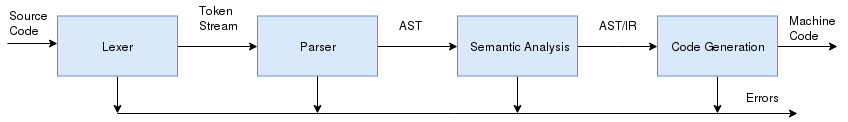
\includegraphics[width=\textwidth]{images/Compilation-process.png}
    \caption{Standard Compilation Process}
    \label{fig:comp_proc}
\end{figure}
% ast main form of code that is operated on 
% has most info flexible for transformation of the output of any stage  
% explain every step
% An appropriate representation of the source code is required to perform the transformations.
The source code takes many different forms as is it passed through the compile process shown above. Starting with text, then to a stream of tokens followed by a parse tree then a detailed abstract syntax tree, and finally machine code. 

\begin{figure}[H]
    \begin{subfigure}[b]{0.5\textwidth}
        \centering
        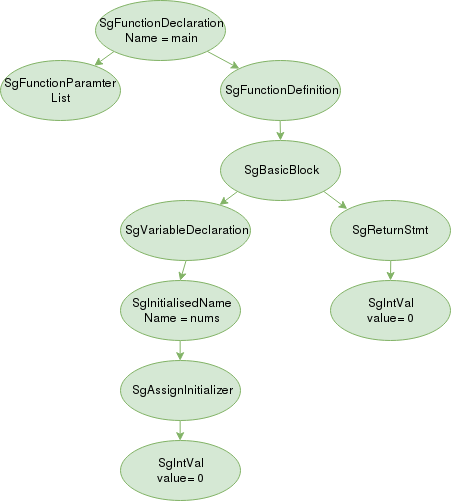
\includegraphics[height=7.2cm]{images/ast-example.png}
        \caption{AST of the function}
        \label{fig:ast-example-AST}
    \end{subfigure}
    \hfill
    \begin{subfigure}[b]{0.5\textwidth}
        \centering
        \begin{minted}{C++}
    int main(){
        int nums = 0;
        return 0;
    }
        \end{minted}
        \caption{Code the AST is representing}
        \label{fig:ast-example-code}
    \end{subfigure}
    \vspace{-0.5cm}
    \caption{Code along side the AST created by Rose Framework }
    \label{fig:ast-example}
\end{figure}

An abstract syntax tree (AST) Figure \ref{fig:ast-example}, an output of the parsing phase, is a representation of the source code used to perform different types of analysis during the "Semantic Analysis" phase. These include type checking, name analysis among others used to create a detailed structure of the code. The AST does not feature any unnecessary punctuation of the input programming, and each node in the tree represents a component of the source code such as a "for loop" or a "variable declaration".

% what is the structure of the tree, class hierarchy of nodes everything is decentdant from type SgNode. 

The abstract syntax tree is also the last form of the source code where it is feasible to obtain a version of the original code. As once the AST has been passed to the code generator too much information is lost(cite), and the original source code cannot be reconstructed in any meaningful way. The AST also stores enough information about the types used by expressions and the scoping of variables for transforms that depend on this information to be executed. The previously mentioned properties make the AST the desirable format for transformations of the source code. 

\begin{figure}[!h]
    \centering
    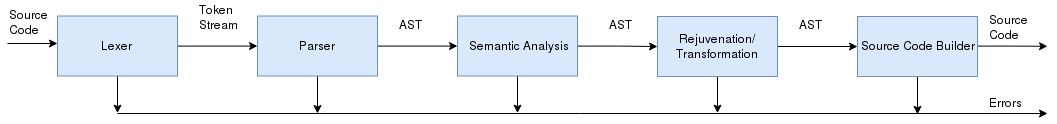
\includegraphics[width=\textwidth]{images/Compilation-process-src.png}
    \caption{Source to Source Compilation}
    \label{fig:comp_proc_src}
\end{figure}

A compiler that is capable of taking the AST, re-parsing it, and outputting source code is called a source-to-source compiler. These compilers can be utilised for many different tasks, such as parallelising "for loops" to make them run efficiently on multiple processor hardware. They are a small fraction of the total set of compilers but remain an evolving research area. Figure \ref{fig:comp_proc_src} shows a brief layout of how the rejuvenations are applied when utilising a source to source compile process. The specific source-to-source compiler framework utilised in the project is explored in the next section.

% what is the output at the different stages explain them why abstract syntax tree is the most feasible output to operate on 
% what is actually transformed ? (AST)
% explored in the next section is the source to source compiler utilised in the project.

\section{Chosen compiler framework: ROSE}
% what is the rose compiler?
\subsection{Rose framework}
The Rose compiler \cite{ROSE} is an open source compiler framework from the Lawrence Livermore National Laboratory (LLNL), it has been utilised to build a range of source to source transformation and code analysis tools \cite{ROSE_TOOLS}. Rose supports a range of languages including Java, C, C++, FORTRAN, Python, and PHP. 
% how does it achieve src to src compilation

It utilises the EDG Front-end \cite{EDG} for parsing C/C++, from there it builds the abstract syntax tree for the source code. Due to the number of supported languages, this acts more like an internal representation than a direct AST for C++. Another feature separating Rose from compilers such as GCC is that it stores additional information such as comments in the AST. This is critical as we want to be able to output code that matches the original as closely as possible. Rose is able to facilitate the rebuilding of the source code through the un-parser component of the framework. As the AST does not store formatting information such as uses of spaces or tabs this has to be specified by the user in formatting options for the output of the code.

Tools utilising the Rose framework are built by first including the necessary header which allows the programmer to call the rose frontend. The frontend takes the file name along with additional options and the framework parses and builds the AST of the source file, outputting a project object as the root of the AST, Figure \ref{fig:trav-proj}. The framework exposes a set of traversal methods which allow for the AST created by the frontend to be traversed. These methods include classical visitor pattern methods but also more simplistic but powerful traversals. 

\subsection{Key Features}

The framework offers a range of methods for accessing data about nodes during traversal, such as type information, links to the declaration of variables from uses, etc. Also supplied is a builder interface, SageBuilder, which simplifies the process of creating new components of code like variable declaration or methods call. These new components can be inserted into the tree by functions such as \textit{prependStatement} and \textit{insertStatementBefore}, which a part of the SageInterface module. 


\subsection{Utilising Rose} \label{UTIL_ROSE}

A simple description of how Rose is utilised is as follows. The transformations to be described in this report are built from extending existing traversal classes such as  \texttt{AstSimpleProcessing} \cite{ROSE_MANUAL} which, unlike the classical visitor traversals, only has a single function \texttt{void visit(SgNode* node)} instead of a function for every type of node. The \texttt{AstSimpleProcessing} is passed an arguement of \texttt{SgNode* node} which corresponds to the current node in the traversal and is passed with the most general possible type that all nodes inherit from SgNode. The programmer is then left to decipher what type the node actually represents. The traversal pass, representing the transform, is instantiated and is passed the root node of the AST. Then by utilising the facilities of the framework described above the rejuvenation is applied at appropriate areas during the traversal. Once the transformation pass is complete the root node of AST is passed to the backend of the rose framework to unparse it, reforming the rejuvenated AST into a human-readable form.    

\begin{figure}[!h]
    \centering
    \begin{minted}{C++}
    SgProject* project = frontend(argv)
    SimpleVarDecTraversal traversal;
    traversal.traverseInputFiles(project, preorder);
    return backend(project);
    \end{minted}
    \caption{Framework utilised for traversal}
    \label{fig:trav-proj}
\end{figure}

The result of writing the transforms in this manner is a single binary that required just the rose library to be installed to run. The tool produced can be operated similarly to other compilers by passing the file to be transformed from the command line.

\begin{figure}[!h]
    \centering
    \begin{minted}{shell}
            modernize-auto test.cpp -o rej-test.cpp
    \end{minted}
    \caption{Command line tool interface}
    \label{fig:cmd-opt}
\end{figure}

% clearly state what is handled by the compiler and how transformations are written
    % linking of the rose library 
    % what is exposes to the programmer to traverse the AST
    % what facilities it has for transforming the AST.
    % how transform are made
    % build system requires linking the 
    
\subsection{Why Rose over Clang}
The Rose framework is not unique among compiler frameworks, others do offer source to source compiling functionality. The most notable of these would be Clang \cite{CLANG}, a compiler front-end for the C family of languages. It utilises the LLVM compiler infrastructure as a back-end and has been used to produce a number of analytical tools \cite{CLANG_TOOLS}. 

Clang was not chosen for this project for a number of reasons, a summary of these can be seen in Table \ref{tab:cmp-rose-clang}. As the table states the Clang front end utilises an immutable AST which means that no alteration to it can occur after parsing. Requiring changes the AST to be text base replacements of the source code, then to reparse the new source code to generate a new AST. This was seen as a disadvantaged compared to the Rose framework allowing direct modification of the AST but does increase the chance of bugs from wrongly manipulating memory. The ways in which clang and Rose framework how programmers to create tools differs. Rose framework allows the programmer to link against the rose framework library \textit{librose} to build the tool completely separated from the Rose framework source code. Clang, however, facilitates both building tools within the source tree and outside with the use of the \textit{libtooling} \cite{CLANG_TOOLS_LIB} but both methods introduce significant work compared to the Rose framework method \cite{ROSE_MAKE}.

\begin{table}[h]
    \begin{center}
        \begin{tabular}{| l | l |}
            \hline
             \textbf{Rose Compiler}               & \textbf{Clang/LLVM}                 \\ \hline
             Rewrites are applied directly to AST & Text bases rewrites (immutable AST) \\ \hline
             Rewrites done by traversing AST      & AST matcher functions               \\ 
             (Visitor Pattern)                    & (pattern matching)                  \\ \hline
             No attempts at modernisation         & Clang-Tidy has modernisation checks \\ \hline
             Good Documentation                   & Better Documentation                \\ \hline
             Build standalone tools easily        & Tools Require work to build/maintain\\ \hline
        \end{tabular}
        \caption{Comparison between Rose and Clang }
        \label{tab:cmp-rose-clang}
    \end{center}
\end{table}
    
% rewrite mechanism for clang seems to be changing and information and tutorial like information seems low 

% offer classical visitor patterns but pushes use of matchers
% The rewrite 

% clang/llvm what is it, brief
% does already have existing tools
% ast rewrites already  

\subsection{Limitation of Rose framework}
In utilising Rose framework certain idiosyncrasies were found that introduce problems in transformed source code. The use of the EDG front-end for parsing C++ results in the expansion of templated types, meaning the default arguments that are usually hidden are present. Resulting in harder to read type signatures when the resulting AST was un-parsed as shown in Figure \ref{fig:temp-expand}. 

\begin{figure}[H]
    \centering
    \begin{subfigure}[h]{\textwidth}
        \centering
        \begin{minted}{C++}
                        std::vector<int> vec;
        \end{minted}
        \caption{Before expansion}
        \label{fig:temp-expand-before}
        \vspace{0.40cm}
    \end{subfigure}
    \begin{subfigure}[h]{\textwidth}
        \centering
        \begin{minted}{C++}
    std::vector< int  , class std::allocator< int  >  > vec;
        \end{minted}
        \caption{After expansion}
        \label{fig:temp-expand-after}
    \end{subfigure}
    
    \caption{Template Type Expansion: Before and After}
    \label{fig:temp-expand}
\end{figure}

There are a number of smaller ways that the transformed source code can differ from the original code, most are harmless and are equivalent to the original. An example of this divergence are lists of initialisations of variables. The variables all being defined with the same type get broken up into individual declaration statements explicitly stating the type as shown in Figure \ref{fig:list-init}. Another smaller occurrence is the deference of variables with calls to methods, \texttt{(*p).q}, is replaced with the more direct arrow notation, \texttt{p$\rightarrow$q}, which is fine as they are semantically the same but may annoy users if not expected. 

\begin{figure}[!h]
    \centering
    \begin{subfigure}[h]{\textwidth}
        \centering
        \begin{minted}{C++}
                            int a, b, c;
        \end{minted}
        \caption{Before expansion}
        \label{fig:list-init-before}
        \vspace{0.40cm}
    \end{subfigure}
    \begin{subfigure}[h]{\textwidth}
        \centering
        \begin{minted}{C++}
                        int a; int b; int c;
        \end{minted}
        \caption{After expansion}
        \label{fig:list-init-after}
    \end{subfigure}
    \caption{List initialisation: Before and After}
    \label{fig:list-init}
\end{figure}

As previously stated, the output style format of the code needs to be specified by the programmer, but the options exposed do not give much control over the desired output. Only allowing for the setting of indentation and if tabs or space are to be used. External tools know as code formatters or pretty printers are well established and are more likely a good choice to reformat the code after the transformation has been applied.

\section{Related work}
% number of tools, what they are for. areas that will be talked about 
There exist a number of tools to aid in the development of software by suggesting or implementing transformations. Code Re-factoring \cite{REFACTOR} is a well-versed area with a lot of integration with modern development environments. Even though refactoring has a different underlying philosophy to altering code as discussed in Section \ref{Introduction} its mission is similar to this project. Another related tool is clang-tidy created by the Clang front-end developers that follow a similar ideology to altering the code as transforms presented in this project. Both refactoring approaches and clang-tidy are discussed in this subsection.

\subsection{Clang-tidy}\label{sec:rw-clang-tidy}
Clang-tidy \cite{CLANG_TIDY} is a clang tool that features numerous sets of static analysis checks for a variety of areas. These include checks for bug-prone code constructs, coherence to a wide range of coding conventions and checking for performance related issues. Clang-tidy also features a set of checks called modernize checks, that target the same style of rejuvenations as mentioned in this project. The clangs modernize checks assess where new C++11 and higher features could be used in place of other methods in the source code. The checks include the likes of "modernize-use-nullptr" which searches for uses of the old keyword \textit{NULL} and replaces them which the C++11 keyword \texttt{nullptr}.

Most of the modernisation passes present in clang tidy focus on changes that do not drastically affect the structure of the code, but there are some which do. The modernize-convert-loop check \cite{FOR_CONVERT} for instance does detects "for loops" of the form \texttt{for( \\declaration; comparison; Increment)} and checks that they are valid to be transformed to "ranged for" of  form \texttt{for( declaration : container)}. Though most checks do not go as far as the loop convert in reconstructing code. As other checks such as modernize-avoid-c-arrays \cite{ARRAY_CONVERT} exist, but it only detects the use of the C array and suggests to use standard library \textit{array} implementation. Modernize-avoid-c-arrays does not attempt to actively fix the problem as the documentation states "it is to difficult to ensure a safe transformation" \cite{ARRAY_CONVERT}. The level of rejuvenation possible is a wider field than just what clang tidy is targeting. Transforms that raise the level of abstraction of user-defined data structures like linked list are yet to be implemented in a modernisation check, as well as other transforms that require spanning checks of the AST.   

\subsection{IDE: tools}
The motivation of code refactoring is centred around creating cleaner and more accessible code without changing the underlying semantics. In contrast, rejuvenation is willing to change what the code actually does to get closer to the programmers intent. Even though they are ideologically different it is still of interest to discuss how far refactoring goes and how people utilise it.

Most modern integrated development environments feature refactoring options that aim to aid developers to increase the maintainability and reduce the complexity of there code. The Popular code editor IntelliJ IDEA \cite{IDEA} includes refactoring methods such as field encapsulation \cite{IDEA_ENCAP} for classes, which creates functions called getters and setters to facilitate access to the variable. Another refactoring method IntelliJ offers is the extract variable  \cite{IDEA_EXTRACT} method which can simplify the complex conditions for "if statements" by extracting and storing parts of the condition into variables to improve readability.

Refactoring, as shown by the condition extraction, does not shy away from altering code, even if this means creating new variable or functions in the case of function extraction. The extent to which refactoring goes is only to change the structure, not the underlying behaviour of the code, so the goals of the two approaches, rejuvenation and refactoring, are distinct. The level of integration refactoring has with IDEs has helped it become widely adopted by programmers and if rejuvenation tools are to become part of the development process, it will be essential to integrate into to IDEs as well.

% list academic papers like the 

% ease of use for developers, interactive
%  extend of actually code manipulation 

%  ========================================= CHAPTER AUTO REJUV =======================================

\chapter{Transform to Utilise Automated Type Inference}\label{chp:auto-tranform}
This Chapter discusses the first source code rejuvenation of the report, which promotes the use of type inference. An explanation of the rejuvenation will be given along with the break down of the conceptual challenges the transform presents. An overview of the implementation is presented showing how the rejuvenation utilised the Rose framework to realise the transform. Finally, an evaluation of the pass and where improvements could be made is used to conclude.

\section{Introduction}
Type inference is a mechanism that enables the type of an expression to be deduced without needing to be explicitly stated,. In the case of variable declaration \texttt{int x = 5}, this could become simply \texttt{x = 5}. Type inference has the benefit of reducing programmer time spend typing laborious type signature, that may even be redundant based on the context surrounding the code. 

%  why it is good

Starting with the C++11 standard, the language introduced type inference through the use of the \texttt{auto} keyword. This implementation of type inference it limited compared to other languages such as Haskell \cite{LYAHFGG_Lipovaca}, as C++ \texttt{auto} can only be used for variable declarations. Unlike C++, Haskell's classical Hindley-Milner type inference allows for the complex type signatures of functions to be inferred from the body of the function \cite{HASK_TYPE_INF}. Figure \ref{fig:auto-type} is an example  showing  how some type signatures can be quite arduous, while not displaying any more useful information than stating the variable is an iterator.

\begin{figure}[!h]
    \centering
    \begin{subfigure}[h]{\textwidth}
        \centering
        \begin{minted}{C++}
std::vector<std::string>::iterator iterName = studentNames.begin();
        \end{minted}
        \caption{Standard type signature}
        \label{fig:auto-type-before}
    \end{subfigure}
    \begin{subfigure}[h]{\textwidth}
        \centering
        \vspace{0.2cm}
        \begin{minted}{C++}
                auto iterName = studentNames.begin(); 
        \end{minted}
        \caption{Infered type signature}
        \label{fig:auto-type-after}
    \end{subfigure}
    \caption{Example of type inference using the \texttt{auto} keyword}
    \label{fig:auto-type}
\end{figure}

The rejuvenation aims to transform type signatures of variable declarations to use the \texttt{auto} keyword in their place. Also ensuring that the variable's type is the same as stated by the original programmer without \texttt{auto} inferring, by mistake, a different type.

% what is type inference how does c++ achieve it
% why the transform makes sense

\section{Conceptual challenges and solutions}
% what does the transformation target
% what exact type of declarations was altered / the focus of transform
    % variable declarations, 
The first conceptual problem that had to be addressed was the scope of the transform, which types of statements would be deemed appropriate for transformation. As stated earlier, C++11 only allows for \texttt{auto} keyword to be used only on variable declarations but this is still a wide expanse of constructs. There exists a number of ways to initialise variables in C++, including initialiser lists for arrays, constructor initialiser, braced initialiser. The focus will be on assign initialiser as constructor initialisers are not supported by C++ \texttt{auto}, and initialiser lists are not altered as type wrongly inferred will be of \texttt{std::initializer\_list<T>}. Assign initialiser are variable declarations that use an equals operator and feature a right-hand side expression, as shown in Figure \ref{fig:ass-var}.

\begin{figure}[!h]
    \begin{minted}{C++}
            vector<string> names = vector<string>(10);
    \end{minted}
    \caption{Assignment intitialiser variable declaration}
    \label{fig:ass-var}
\end{figure}

% What had to be ignored 
    % initialiser lists
    % Class fields
\subsection{Type Modifiers}
In approaching the problem it was essential to take type modifier into account as they play an important roll in specifying types. These modifiers are the terms that add additional meaning and constraints on to uses of variables. Modifiers include \textit{const}, ampersand operator \&, Pointer astrix *, \textit{volatile}. The transform had to handle each of these modifiers carefully to preserve the proper meaning of the code. 

Const and reference operators need to be kept the same if utilised, as they apply different properties to the type that \texttt{auto} can not infer from the right-hand side. How this type information is preserved is discussed in the implementation section. 

\subsection{Pointers}
% pointer and the decision on how to handle them 
There was a decision to be made with the use of pointers in the type annotation as \texttt{auto} is capable of inferring the use of pointers, but also capable of having them present alongside as shown in Figure \ref{fig:ptr_type_inf}. It was decided that pointers should always be inferred by \texttt{auto} due to the cleaner look of the type signature. 

\begin{figure}[!h]
    \centering
    \begin{minted}{C++}
                auto ptrToCat = getCatObj();
                auto *prtToCat = getCatObj();
    \end{minted}
    \caption{Equivalent type signature with pointer inference}
    \label{fig:ptr_type_inf}
\end{figure}

% \begin{figure}[!h]
%     \centering
%     \begin{subfigure}[h]{\textwidth}
%         \centering
%         \begin{minted}{C++}
%                 auto ptrToCat = getCatObj();
%         \end{minted}
%         \caption{Version 1}
%         \label{fig:ptr_type_inf-1}
%         \vspace{0.40cm}
%     \end{subfigure}
%     \begin{subfigure}[h]{\textwidth}
%         \centering
%         \begin{minted}{C++}
%                 auto *prtToCat = getCatObj() 
%         \end{minted}
%         \caption{Version 2}
%         \label{fig:ptr_type_inf-2}
%     \end{subfigure}
%     \caption{Equivalent type signature with pointer inference}
%     \label{fig:ptr_type_inf}
% \end{figure}

% const and reference operators
%  what about them that they are still there

\subsection{Implicit Casting} \label{sect:con-impl-cast}
% implicit casting needs to be handled
An important component of the C++ type system is implicit casting, which raises problems when inferring types with \texttt{auto}. An implicit cast is created when the type signature does not match the type presented on the right-hand side of the assign statement, and the typecasting is valid. If \texttt{auto} was applied blindly in this situation then the casting would be lost and only the type expressed on the right-hand side would be inferred. These changes can be quite subtle, as shown in Figure \ref{fig:implicit-cast}. The unsigned type signature will not be inferred from the integer on the right, as its base type is \texttt{int} not \texttt{unsigned int}. The use of type \texttt{int} instead of \texttt{unsigned int} could lead to unexpected overflow errors, which were not previously there. The situation could be rectified by adding an explicit cast on to the right-hand side but this would not benefit the readability of the code as the type has just moved from the left-hand side to the right. Therefore it was decided that variable declarations using implicit casts would not have the type signatures altered.   

\begin{figure}[!h]
    \centering
    \begin{subfigure}[h]{\textwidth}
        \centering
        \begin{minted}{C++}
                unsigned int counter = 0;
        \end{minted}
        \caption{Before: type declared, unsigned int}
        \label{fig:implicit-cast-before}
        \vspace{0.40cm}
    \end{subfigure}
    \begin{subfigure}[h]{\textwidth}
        \centering
        \begin{minted}{C++}
                auto counter = 0; 
        \end{minted}
        \caption{After: type inferred, signed int}
        \label{fig:implicit-cast-after}
    \end{subfigure}
    \caption{Hazards of implicit casting, unsigned type \\ lost when inferring with auto}
    \label{fig:implicit-cast}
\end{figure}

% extent to which types are replaced
    % any var dec could be changed disregarding the length of the type.
\subsection{Scope of Transformation}\label{sec:auto-scop-trans}
A naive approach for applying the \texttt{auto} rejuvenation is to replace every valid variable declaration's type with \texttt{auto}, but this is not always advisable. As some types are short, such as the inbuilt types, it would not improve the code in a measurable way if these type annotations were replaced. Also, a factor to be considered is that type annotations offer insightful information that is not immediately revealed from the right-hand side of the declaration. With the use of \texttt{auto}, it may require more work by the programmer to decipher what the code is trying to do. This is not an intrinsic problem with using \texttt{auto} but a result of not using appropriate names for variables and objects when declaring them, the problem can be mitigated by utilising good coding conventions. 

The approach used for the conditions to replace type signatures is naive, aiming to replace all instances where applicable. The slightly more advanced approach implements a lower bound on the character length of the type to be replaced. So that shorter types do not end up unnecessarily changed or even made long in the case of type \texttt{int}.

\section{Implementation}\label{sec:auto-Impl}

\subsection{Valid Variable Declaration}
The rejuvenation is centred around a single pass of the AST with only the input files being traversed, not the files present in include statements. After the source code is parsed by the Rose framework, line 1 of Figure \ref{fig:trav-proj}, the AST is traversed by the VarDecTraversal class which inherits from the AstSimpleProcessing discussed in Section \ref{UTIL_ROSE}. The traversals \texttt{visit()} method is passed each node in the AST and is the main entry point for the auto modernisation transform that was built.

The desired node as a starting point for the transform is the \textit{InitializedName} node Figure \ref{fig:var-dec-ast}, as this is the node that stores the associated name of a variable declaration along with its type. The framework features a run time type information (RTTI) system for deciding if nodes are of specific types, such that if we wanted to find if the current node is a \textit{SgInitializedName} we use the \textit{isSgInitializedName(node)} function.

\begin{figure}[H]
    \centering
    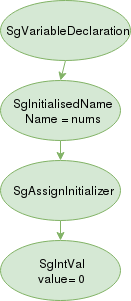
\includegraphics[height=6cm]{images/ast-var-dec.png}
    \caption{AST of variable declaration, \texttt{int nums = 0}}
    \label{fig:var-dec-ast}
\end{figure}

After the current node is checked to be of type IntializedName, the transform checks for a number of other properties. Nodes that are generated by the compiler, instantiated template code, could include IntializedName nodes so these are filters out by checking the method \texttt{isCompilerGenerated()} of the node. The IntializedName node stores a pointer to the associated initialiser type, this is checked to ensure it is of type SgAssignInitializer ensuring it does feature an expression on the right-hand side of an equals operator. A further restriction on \texttt{auto} is that is cannot be utilised for non-static class fields. So the parent of the Variable Declaration, which is the parent to the InitializedName Figure \ref{fig:var-dec-ast}, is checked to ensure the variable declaration does not take place in class as a field. The parent of the InitialisedName node is checked to be a Variable Declaration as a sanity check to ensure InitalisedName is not associated with anything but a declaration. 

Once the variable declaration has been found, call an internal method of the InitialisedName node to see if it is already utilising \texttt{auto}, and return from the function if true, moving on to the next node in the AST. 

It is at this stage in the process implicit casting of types can be checked. As the framework utilises SgCastExpr nodes to express the use of casting in the code, we can check the right-hand side of the assign statement for the presence of this node. To check what kind of expression is on the right-hand side requires using the \texttt{get\_operand()} of the AssignInitiailizer node to return the root expression node. To be able to differentiate between implicit and explicit casts the transform has to not only check that the node is SgCastExpr, but that it is also compiler generated. As the compiler inserts the SgCastExpr to the head of the expression tree in the case of an implicit cast. If both conditions are met the transform returns from the visit function, and moving to the next variable declaration without altering the type signature as stated in Section \ref{sect:con-impl-cast}. 
% pseudocode implicit cast 

\begin{figure}[!h]
    \centering
    \begin{minted}{python}
    rhsExpression = initializerAssignNode->get_operand()
    if (isCastNode(rhsExpression) and 
            rhsExpression->isCompilerGenerated() )
        return;
    \end{minted}
    \caption{Psuedocode for implicit casting check}
    \label{fig:cast-check-code}
\end{figure}

% 0. addition traversing only the input files !
% 1. filtering the nodes !
% 4. checking for auto already !
% 3. filtering of implicit cast checking for compiler generators 

\subsection{Transforming Type Declaration}
After we have performed all the above checks the variable declaration is allowed to be transformed. We replace the existing type with is a SgTemplateType initialised with the name \texttt{auto}, as there does not exist a type for \texttt{auto} within the SgType class structure. 

The transform cannot blindly replace the existing type with \texttt{auto} as doing so would remove all additional type information, \textit{const}, pointers, and other keywords. Types that are built up of the previously mentioned types are called nested types, as they store a pointer to the type that is stored inside of it, with the deepest type being the base type.
% add figure

So to distinguish between the cases where nested types are used the framework provides a method \textit{containsInternalTypes()} which returns a boolean and is present in all type nodes. This was used in conjunction with the \textit{get\_type()} of the InitializedName node to get the type of the variable being declared. For the case where the type of the IntitialisedName node did not contain nested types, we could simply replace the pointer to the type node with the \texttt{auto} SgTemplateType. 

\begin{figure}[H]
    \centering
    \begin{minted}{python}
    if ( varDecType->containsInternalTypes())
        typeCopy = varDecType->copy()
        setbaseType(typeCopy, SgTemplateType("auto"))
        typeCopy->stripType(POINTER_TYPE)
        assignNode->set_type(typeCopy)
    else
        assignNode->set_type( SgTemplateType("auto"))
    
    \end{minted}
    \caption{Psuedocode: Setting type Declaration}
    \label{fig:auto-cases-nested-types}
\end{figure}

In the case of nested types, the code is not as simple, as the types could be nested to an arbitrary depth. The framework does offer \textit{find\_base\_type()} and \textit{set\_base\_type()} methods for types, but utilising them directly resulted in unexpected behaviour. If the methods are utilised directly then any expression that also utilises the type will have its type replaced with the \texttt{auto}. For example, if a variable \textit{b} is a reference to a variable \textit{a} with the type of \textit{a} being SgTypeInt then the base type of \textit{b}, SgTypeInt, is actually linked to \textit{a} and is shared. This comes about due to the types acting more as a graph leading to sharing of type information. So if the base type of \textit{b} is changed then \textit{a} is also changed. In the case shown in Figure \ref{fig:type-con-bug} this is not harmful but this can also occur for function parameters. So in changing a variable declaration to \texttt{auto} a function parameter also linked to that base type will also change to using \texttt{auto}, \texttt{foo(auto x, string b)}, which is an invalid use of \texttt{auto}.

\begin{figure}[!h]
    \begin{minted}{C++}
                        int a = 10;
                        int &b = 5;  
    \end{minted}
    \caption{Type connection in AST/Graph structure}
    \centering
    \label{fig:type-con-bug}
\end{figure}

\subsection{Locating Base Type}\label{sec:auto-loc-base-type}


As variables, functions, etc can hold pointers to the same type node in a graph like structure type nodes cannot be changed without unintentionally altering other statements that point to them. So to void this problem from occurring the transform had to replicate type nodes, which could be nested, before altering them. The framework does feature facilities for performing a deep copy which copies entire subtree not just the first node of the AST. As the type information is not represented in the AST model and is only present in larger graph structure of the program this deep copy has to be manually applied at each nested type to build a cop, see Figure \ref{fig:code-set-type}. 

This approach of recursing down the nested type, and copying each node to build a complete copy is achieved by a function \texttt{setBaseType()}, Figure \ref{fig:code-set-type}, created for the transform. A while loop checks if the type contains internal types at each stage build the copied type as it goes. At the deepest level, the type without any further nesting the type is replaced with the \texttt{auto} type. 

% remember to strip pointers

\begin{figure}[H]
    \begin{minted}{python}
    def setBaseType(typeVar, newBaseType)
        while (typeVar->containesInternalTypes()):
            prev_type = typeVar
            typeVar = typeVar->get_interal_type()
            typeVar = typeVar->copy()
            prev_type->set_type(typeVar)
        prev_type->set_type(newBaseType)    
            
    \end{minted}
    \caption{Pseudocode: setBaseType}
    \centering
    \label{fig:code-set-type}
\end{figure}

Upon returning from the \texttt{setBaseType()} function the type passed to it as \texttt{typeVar} is now a copy of the original type with the deepest type set to \texttt{auto}. The copied type with \texttt{auto} set still has all of its additional type modifiers, including pointers which \texttt{auto} could helpfully infer. So before the altered type replaces that of variable declaration the pointers are stripped from the type, Figure \ref{fig:cast-check-code}. 

% ----------------------------------------------------------------
% 2. build replacement type 
% 5. main checking for internal types
% 6. if no internal types replace type 
%   failure to find base type -_- 
%   graph structure of types
%       functions parameters
% 7. if yes why do we need to recurse the data structures
    % recursive function to base type
% ------------------------------------------------------------------

% How the transform was implemented 
    % template type without


% compiler generated code 

% problems faced 
    % recursive type definitions 
    % linking of type information present in the memory graph (function args changing type)
    
    
% notation of internal types linking in a graph structure 
\section{Evaluation} % Critical evaluation of own work

\subsection{Problems encountered in development}
% intro link back
% type system how it was hard to work with how it was finally figured out (graph) 

The Implementation of the transform portrayed in Section \ref{sec:auto-Impl} is significantly smaller than the for-loop rejuvenation discussed in Section \ref{chp:loop-transform}. but this does not mean the implementation was anymore straight forward. As the transform focused on altering types, the complex nature of the C++ type system meant many problems faced did not have a clear root cause or solution. 

A major hurdle faced when trying to work with nested types was discussed in Section \ref{sec:auto-loc-base-type}, with the linking type nodes across different uses. The effect of altering types of variable declaration, function arguments or other structures directly through pointers to type nodes was extremely hazardous due to this linking. The problem in debugging this incorrect type alteration was increased due to rose documentation not stating how types were utilised in the AST. The connection between types and where they are used was only made clear when the graph representation of the source code was viewed. The graph of the source code features extra attributes and links which includes type nodes and their connection not shown in the normal AST. The graphs can be created by a command line tool built by the Rose Framework developers \textit{dotGeneratorWholeASTGraph} \cite{ROSE_TUT} which takes the source code and create a dot file that can be displayed as a graph.

Even though the Rose framework has functions and methods for retrieving and altering types, it is clear they are not of a high enough abstraction to be used without close consideration.

\subsection{Limitations and critique of transform} 

% usefulness, transform may not really aide in readability, changing types on normal variables may make them more cryptic, use of auto may come down to a subjective choice. 

The transform was designed to target every assign type variable declaration without much thought to the usefulness of changing the type to \texttt{auto}. This changing of the type can be undesirable in many cases as the type could give much-needed context to the variable being declared. 

As stated in Section \ref{sec:auto-scop-trans}, strict adherence to a coding convention for naming variable could allow for \texttt{auto} to infer the type without decreasing the readability. However, if this coding convention required manual changes to the code it would completely nullify the automated aspect of the rejuvenation. There could be an automated process to assess if the variable name has enough information represented in the type but this would be a very complex solution. A simpler and more effective approach would be to restrict or reduce the scope of the transform to places where type information is definitely duplicated.

% overly applied transform, many cases not yet checked which could cause problems as transform it not conservative in nature

As stated above the transform is not design to be conservative as it tries to alter every variable declaration. It was seen during testing on real-world code examples that this is a very error-prone approach as the complexity of the C++ language leads to many unforeseen cases where the transform fail unexpectedly. To create a production-ready version of the tool in this form would require significant testing or alter it to target more specific use cases of \texttt{auto} type inference.

\subsection{Comparison to Clang-tidy \& Testing }\label{sec:cmp-auto-reju-mod-auto}

% intro Of these modernize checks the modernize-use-auto \cite{}

As discussed in related work, Section \ref{sec:rw-clang-tidy}, clang-tidy features many static analysis checks with some categorised as modernizing checks. The modernize-use-auto \cite{CLANG_AUTO} is the most relevant to compare against as it also tries to promote the use of type inference using auto. Clang-tidy's modernize-use-auto does differ in several significant ways as it does not try to transform all variable declarations. It chooses to focus on transforming variables that are declaring iterators of the standard container classes, e.g list, vector. Also replaces types with auto when the variable being declared uses the new operator on the right hand, Figure \ref{fig:code-new-vardec}. The final case it can transform is when any form of casting is utilised such as old c-style casting, or the newer templated function style casting, Figure \ref{fig:code-modern-cast}.

\begin{figure}[H]
    \begin{minted}{c++}
                NameOfType* ptrToObj = new NameOfType(); 
    \end{minted}
    \caption{Varible Declaration using \texttt{new} operator}
    \centering
    \label{fig:code-new-vardec}
\end{figure}

\begin{figure}[H]
    \begin{minted}{c++}
    unsigned int res = static_cast<unsigned int>(getCount());
    \end{minted}
    \caption{Example of Modern C++ cast}
    \centering
    \label{fig:code-modern-cast}
\end{figure}

The difference in the targets of the transformations complicates the comparison of the two tools. In contrasting the two approaches, clang takes a more focused approach which lends its self to more controlled transformation,  mitigating problems with the unexpected code being transformed.

For testing of the auto-rejuvenation tool, produced by in the project, benchmarks were selected from real code bases as well from the benchmarks already present in the SPEC CPU benchmarks \cite{SPEC}. The Benchmarks include the single header libraries Nanoflann \cite{blanco2014nanoflann} and Swarmz \cite{SWARMZ} as well as files included in the 541.leela\_r \cite{SPEC_LEELA} SPEC benchmark.

% ================== FIX ME =======================
% , and 531.deepsjeng\_r \cite{SPEC_DEEPSJENG}.
 
The data collected from running auto-rejuvenation and clang-tidy's modernize-use-auto on the benchmarks, Table \ref{tab:auto-tool-benchmark-res}, shows the disparity in two approaches. The effect of modernize-use-auto's selective cases for transformation can be seen by its near-zero number of transforms on the benchmarks. Even with this low hit rate, it does not say much about the effectiveness of the tool as it is aiming to help only where it knows it can reduce type duplication. In comparison the high hit rate of the auto tool is also misleading as a sign of effectiveness, as many of the transformations are on simple base type definitions such as \texttt{int} or \texttt{bool}. Transforming basic types does not increase readability of the code, and for types like \texttt{int} actually increases the length of the type signature. There also is the problem of if every variable should utilise \texttt{auto} which is most likely not the case, but individual case by case checking is complex.   

% The selective nature of clang show in this small data set, not bad, on the other hand high counts for auto-rejuventation is misleading as a sign of improvement as many of the transformation or on base types with small type signatures.

%  table here
\begin{table}[H]
    \begin{center}
        \begin{tabular}{| l | l | l | l | l |}
            \hline
            \textbf{Benchmark}    & \textbf{File Name}    & \textbf{\# of lines}  & \textbf{\# of trans,} & \textbf{\# of trans,} \\ 
                                  &                       &                       & \textbf{auto-rejuv}   & \textbf{clang-tidy}   \\ \hline
            Nanoflann    & nannoflann.cpp   & 2042  & 10  & 0\\ \hline
            Swarmz       & swarmz.cpp.cpp   & 344   & 42  & 0\\ \hline
            541.leela\_r & FastBoard.cpp    & 2452    & 217 & 0\\ \hline
                         & GTP.cpp          & 502    & 22  & 0\\ \hline
                         & UCTSearch.cpp    & 469   & 39  & 0\\ \hline
                         & UCTNode.cpp        & 457   & 28  & 0\\ \hline
        \end{tabular}
        \caption{Benchmark results for auto-rejuvenation and modernize-use-auto}
        \label{tab:auto-tool-benchmark-res}
    \end{center}
\end{table}

Further insights into the types being transformed by auto-rejuvenation can be seen when the minimum type length to be transformed was set to 6, Table \ref{tab:auto-tool-benchmark-type-limit}. A minimum length of 6 works well for filtering basic types as most of the basic types have 5 or fewer characters, which would not benefit from increased readability. The notable decreases in the number of transformations when compared to the previous tests in Table \ref{tab:auto-tool-benchmark-res} shows that being more selective is required if meaningful uses of auto are to be introduced automatically.

% The number of basic types being transformed unnecessarily can be seen when contrasting the table above with Table \ref{tab:auto-tool-benchmark-type-limit}, where the auto-rejuvenation tool has been run with minimum type length to be transformed set to 6. A minimum length of 6 work well for filtering basic types as 

% For further insight into the types being transformed by auto-rejuvenation, when a type length limit is imposed on the types to be transformed in the auto-rejuventation tool is drastically reduced the number transformed. 

% though this does help better methods are need for accessing the usefullness of auto being applied

% table with min name set
\begin{table}[H]
    \begin{center}
        \begin{tabular}{| l | l | l | l |}
            \hline
            \textbf{Benchmark}    & \textbf{File Name}    & \textbf{\# of lines}  & \textbf{\# of trans,} \\
                                  &                       &                       & \textbf{auto-rejuv}   \\ \hline
            Nanoflann    & nannoflann.cpp   & 2042  & 6  \\ \hline
            Swarmz       & swarmz.cpp.cpp   & 344   & 29 \\ \hline
            541.leela\_r & FastBoard.cpp    & 2452	& 13 \\ \hline
                         & GTP.cpp          & 502	& 9  \\ \hline
                         & UCTSearch.cpp    & 469   & 15 \\ \hline
                         & UCTNode.cpp	    & 457   & 11 \\ \hline
        \end{tabular}
        \caption{Benchmark Test data of Project Auto }
        \label{tab:auto-tool-benchmark-type-limit}
    \end{center}
\end{table}

% need a middle ground
It is clear that both approaches do have their respective benefits, but a tool that is more complex selection than auto-rejuvenation, and is more open to transforming than modernize-use-auto is required to fully extract the benefits that \texttt{auto} could bring.

% comparison against clang
% -! operates significant different that the clang tidy tool, does not only focus on std iterators or uses with the new operator 
% -! does not seem willing to handle variable declarations that don't use new but are longer than minimum length
% - has a low hit rate going to be hard to find stuff that utlises it 
% - testing, table of tests talk about why certain points match.

% Results of use (data)

\subsection{Possible Extensions}
In the years following the introduction of \texttt{auto} in C++11, the standards to follow it continued extending the use cases for the keyword. Since the C++14 standard, \texttt{auto} has been able to infer the return types of functions as seen in Figure \ref{fig:funct-ret-inferred}. Extending the auto tool to infer return types of functions would be suitable for simple functions, but for handling all cases of transformation involving complex templated functions a separate tool would be more sensible.

\begin{figure}[!h]
    \centering
    \begin{subfigure}[h]{\textwidth}
        \centering
        \begin{minted}{C++}
                Counter getCounterObj(){
                    return lineCounter;
                }
        \end{minted}
        \caption{Before: type declared, unsigned int}
        \label{fig:funct-ret-inferred-before}
        \vspace{0.40cm}
    \end{subfigure}
    \begin{subfigure}[h]{\textwidth}
        \centering
        \begin{minted}{C++}
                auto getCounterObj(){
                    return lineCounter;
                }
        \end{minted}
        \caption{After: type inferred, signed int}
        \label{fig:funct-ret-inferred-after}
    \end{subfigure}
    \caption{Inferring function return types}
    \label{fig:funct-ret-inferred}
\end{figure}

%  more selective in the way it handles cases (e.g like clang) utilise type information, exentend to allow functions return types to be inferred added c++14 i think 

\section{Summary}% what goes here ? 
This chapter presented the auto-rejuvenation tool, explaining the purpose of type inference and how it can be utilised to rejuvenate source-code. The underlying concepts and focus of the tool were discussed followed by details of the implementation. The tool was then assessed by running it against a set of selected files as a benchmark, as well as contrasting these results with a similar tool, modernize-use-auto, developed by Clang. 

The auto-rejuvenation tool discussed in this chapter was a locally focused transformation. It only dealt with a single line of the source code, a variable declaration, to be transformed in any instance. In the following chapter a more complex and spanning rejuvenation, for loop transformation, will be present. This transformation will require many spanning checks and transformations within the loop's body, as well as more complex methods of removal and insertions into the source code. The for loop transform should reveal more of the power of automated rejuvenation in handling a complex transformation, as the tedious and error-prone work of checking the entire loop body by hand is removed.


% This chapter has... explain what has been presented in this chapter 
% Link to next chapter ... a more elaborate transformation is presented in the next chapter, spanning changes and checks
% Ways it can be extended 

\chapter{Loop Transform: For Loop to Ranged For Loop}\label{chp:loop-transform}

% Abstract for chapter
This Chapter aims to introduce the second rejuvenation of the project, which converts for loops to range-based for loops where appropriate. An Introduction to the use case for ranged-for loops is given along with the benefits they can provide when utilised. Next, the conceptual challenges are discussed, explaining the scope of the traversal and what categories of for-loops are utilised. A more in-depth look at the implementation details is given after with a focus on the multiple traversals used to realise the transformations. To conclude, an evaluation of the for-loop-rejuvenation is given with comparison to an existing clang-tidy tool with a discussion of the limitation and extensions that could be made to improve effectiveness.

\section{Introduction}
\subsection{Type of for-loops}
For loop statements are a concept familiar to most programmers and are implemented in most programming languages inspired by C such as Java, C\#, go, perl. In C++, and most other languages, the for statement has three components init-expression, comparison expression and loop expression as seen in Figure \ref{fig:code-for-loop}, though each component is not required and can be a general expression. 

\begin{figure}[H]
    \centering
    \begin{subfigure}[h]{\textwidth}
        \centering
        \begin{minted}{C++}
        for(init-expression; cond-expression; loop-expression)
        \end{minted}
        \caption{Components of C++ for loop}
        \label{fig:code-for-loop-components}
        \vspace{0.40cm}
    \end{subfigure}
    
    \begin{subfigure}[h]{\textwidth}
    \begin{minted}{C++}
                    for(int i = 0; i < 10; i++)
    \end{minted}
    \caption{Example of C++ for loop}
    \centering
    \label{fig:code-for-loop-example}
    \end{subfigure}
    \caption{C++: for loop construct}
    \label{fig:code-for-loop}
\end{figure}

A common use of for loops is to index into arrays or other higher level container abstractions, such as List, Vectors or Sets and utilise each element in the loop body. This use case is so prevalent that C++ introduced the notation of an iterator interface \cite{ITER_CPP} to aide with the traversal of containers, Figure \ref{fig:code-iterator}, where indexing is a more costly operation, as the case with \texttt{std::lists}. 

\begin{figure}[H]
    \begin{minted}{c++}
        for(list<int>::iterator elem = num_l.begin();
                elem != num_l.end(); elem++)
    \end{minted}
    \caption{Iterating through a List}
    \centering
    \label{fig:code-iterator}
\end{figure}

The prevalence of needing to iterate or index through a complete container or array also lead to the introduction of ranged-based for loops, Figure \ref{fig:code-ranged-based-for}, in the C++11 standard \cite{RANGED_FOR_CPP}. Many other languages had implement similar ranged-based for loop before C++, with Java including them since Java 5 \cite{JAVA_RANGE}, and languages like Python and Rust only implementing ranged-based for loops in their languages. Ranged-based for loops use a compact syntax with a variable taking the values of the container on the left hand with the container being iterated on the right, with the two separated by a colon. 

\begin{figure}[H]
    \begin{minted}{c++}
                        for(int elem : num_l)
    \end{minted}
    \caption{Ranged-based for loop over a list}
    \centering
    \label{fig:code-ranged-based-for}
\end{figure}

\subsection{Key differences}

The key difference between standard for-loops and ranged-based is that the loop iterates through the whole container, it can not do partial iterations. Another difference is the ranged-based for loop are more restrictive as only one container can be traversed in the loop, whereas a standard for loop could use its index in multiple arrays or containers, as well as other expressions. 

While is maybe more restrictive, the syntax utilised for ranged-based for loops in Figure \ref{fig:code-ranged-based-for} is very compact and readable compared to standard for loop, Figure \ref{fig:code-for-loop-example}, and even more so than the very verbose syntax for using iterators, Figure \ref{fig:code-iterator}.

% The clean and simple look of the make ranged-based for loops attractive to developers
\subsection{Rejuvenating for-loops}
The rejuvenation developed in this chapter, ranged-for-rejuvenation, aims to transform for loops of the type present in Figures \ref{fig:code-for-loop-example}, \ref{fig:code-iterator} to utilise ranged-based for loops. As the ranged-based for loops can only be used in a specific situation where one container or array is being traversed completely, many uses of for loops would not be valid to transform. What conditions are required for a loop to be transformed are discussed in Section \ref{sec:for-concept}. 

The goal of the transformation is to increase the readability and maintainability of the code, through utilising the simple and more compact range-based for loop to better express the underlying logic of the code. The readability is increased using ranged-for loops as the container which is the focus of the for loop is displayed in the loops header, meaning the programmer is not required to scan the loop to access if the loop is iterating through an array or container.

% what are standard for loops, for (initialiser, comparison, iterator){}
% what are ranged-based for loop
% diff between loops
% how is it a rejuvenation, added in C++11 standard previous way of doing it 
% why is the rejuvenation worth it, what is the benefit ? 
    % more concise notation
    % readability
    % Other languages utilise ranged for a lot e.g python does not even have standard loop
%  examples required


\section{Conceptual challenges and there solutions}\label{sec:for-concept}
\subsection{Scope of transformation}\label{sec:forLoop-scope-trans}
As the number of ways to use a for loop construct is limitless, the transform imposes restrictions on the form the for loops can take. This is to help identify the for-loop type that can be transformed and assess if it can be done safely. The transform, ranged-for-rejuvenation, focuses on three distinct ways of utilising for loops that is tries to transform shown in Figure \ref{fig:code-for-types}. 

The iterating over a container for loop type as shown previously in Figure \ref{fig:code-iterator}, is the first type the transformation attempts to detect.
The conditions for Iterator loop type, Figure \ref{fig:code-for-iter}, being met is that \texttt{CONT} must be a container which utilises the \texttt{begin} and \texttt{end} functions, the type, \texttt{TYPE}, of the container is not checked. The \texttt{it\_name} must also be the same variable across the three components of the for loop, and the cond-expression must be a \texttt{!=} operator, but the position of the arguments does not matter. To be matched to this use case the \texttt{COND} cannot be a reference and the functions calls must directly follow the container. 

\begin{figure}[h]
    \centering
    \begin{subfigure}[h]{\textwidth}
        \centering
        \begin{minted}{C++}
for(TYPE it_name = CONT.begin(); it_name != CONT.end(); it_name++)
        \end{minted}
        \caption{Iterator Loop Type }
        \label{fig:code-for-iter}
        \vspace{0.2cm}
    \end{subfigure}
    
    \begin{subfigure}[h]{\textwidth}
    \begin{minted}{C++}
    for(TYPE idx_NAME = 0; idx_NAME < CONT.size(); idx_NAME++)
    \end{minted}
    \caption{Array-like container Loop Type}
    \centering
    \vspace{0.2cm}
    \label{fig:code-for-container}
    \end{subfigure}

    \begin{subfigure}[h]{\textwidth}
    \begin{minted}{C++}
    for(TYPE idx_NAME = 0; idx_NAME < (([0-9]+)|VAR); idx_NAME++)
    \end{minted}
    \caption{Statically allocated array Loop Type}
    \centering
    \label{fig:code-for-stat}
    \end{subfigure}
    
    \caption{Uses of for loops to transform}
    \label{fig:code-for-types}
\end{figure}


The second loop form attempts to match the use case where an array like container is utilised, meaning a container that is not iterated over but indexed into using array access notation or direct member functions, \texttt{at}. The requirement to match the second for loop, Figure \ref{fig:code-for-container}, are that \texttt{idx\_name} is a variable being declared which is assigned 0, and appears the same throughout the three components. The comparison, cond-expression, requires comparing \texttt{idx\_name} to the container, \texttt{COND}, where \texttt{idx\_name} is required to be less than a method call to function \texttt{size}. Finally the loop-expression of the for loop should be \texttt{idx\_name} in a pre/post increment operation.

The final case, statically allocated arrays, that the transform attempts to transform is shown in figure \ref{fig:code-for-stat}. The init-expression of the for is the same as the previous case, while the cond-expression differs. The comparison is between \texttt{idx\_name} and either a number which matches the size of the allocated array, Figure \ref{fig:code-static-for-cmp-num}, or a \texttt{const} variable which is assigned the same value as the size of the array, Figure \ref{fig:code-static-for-cmp-var}. The variable has to be \texttt{const} to ensure the size is not altered before it is used in the comparison. The comparison allows operator \texttt{!=}, $<$ and $>$ where \texttt{idx\_name} has to be less than size used. 

\begin{figure}[h]
    \centering
    \begin{subfigure}[h]{\textwidth}
        \centering
        \begin{minted}{C++}
                int arr[N];
                const int N = 10;
                for(int i = 0; i < N; i++){...}
        \end{minted}
        \caption{Index loop: comparing against variable}
        \label{fig:code-static-for-cmp-var}
        \vspace{0.40cm}
    \end{subfigure}

    \begin{subfigure}[h]{\textwidth}
    \begin{minted}{C++}
                int arr[10];
                for(int i = 0; i < 10; i++){...}
    \end{minted}
    \caption{Index loop: comparing against value}
    \centering
    \label{fig:code-static-for-cmp-num}
    \end{subfigure}

    \caption{Uses of for loops to transform}
    \label{fig:code-static-for-cm}
\end{figure}

    % 3 types of loops targeted 
        % iterator for loops  
        % container like for loops
        % statically defined arrays 
    % all distinct cases 

\subsection{Loop information extracted}
To perform necessary checks and traversals later in the transformation the container name and variable used in the needed to be extracted. For each for-loop, the transform would check if the loop matches any of the above cases and if so extracts the iterator, \texttt{it\_name}, or index,  \texttt{idx\_name}, from the init-expression. The container can be extracted from the cond-expression in the case of an iterator for loop and the array like for loop, but this is not the case for the statically allocated array, only a value or variable representing the size is present. 

The solution to locating the container utilised by the statically allocated type for-loop was to traversal the loop body to find the array being indexed by the \texttt{idx\_name} variable. The search of the loop body would look for any array access notation and see if the index variable reference was the only expression present, \texttt{arr[idx\_name]}. If more than one array is being indexed the transform does not continue attempting to transform the loop, as ranged for only iterates over one container. If no container is found to be indexed the transform stops and the next for loop is checked.


%     % deciding what type of loop we are dealing with
%         % things that are consistent across the types
%             % index/iterator is required to be the same across all 3 components of for

% Explain difference in container detection for  

\subsection{Safety of transformation}\label{sec:safety-of-trans}
Assessing the safety of the transformation was the next significant challenge to handle, as certain uses of the iterator/index or container/array in the loop body could render the transformation to ranged-for invalid. The cases the transform aims to handle all have distinct ways the index/iterator or container/array are allowed to be used in loop body so are assess separately to assess safety.

\subsubsection{Safety: Iterator loop body}\label{sec:safe-iter}
The iterator for loop case differs from the array-like and statically allocated cases as the index is not a simple integer value, but an iterator that acts as a pointer to the object stored in the container. This means that in the body of the loop the iterator can only be deference directly or by using arrow expression, Figure \ref{fig:code-iter-uses}. If any other operation is performed on the iterator then the transformation is considered invalid as altering the position of the iterator, \texttt{it\_name}, would not map to a full iteration through the container as is the case when using a ranged-for loop. 

\begin{figure}[h]
    \centering
    \begin{minted}{C++}
                                ...
                        *it_name
                        it_name->getField()
                                ...
    \end{minted}
    \caption{Acceptable uses of Iterator in loop body}
    \label{fig:code-iter-uses}
\end{figure}

As the container is not required to be in the loop body to be indexed into, as is the cases for the other for loop types, any use or function call on the container in the loop body invalids the transform. The transform is invalidated as function calls, e.g \texttt{vec.push\_back(item)}, on the container could alter the underlying size of the container which could cause dangerous undefined behaviour when iterating through the transformed ranged-for. This would not necessarily happen but as the ranged-for takes a copy of the length of the array at the initialisation of the loop, any changes to the size of the array would make this copied length of the container outdated and lead the iterator to access invalid or wrong data. 

\subsubsection{Safety: Array like loop body}
The array-like loop type requires additional checks in the loop body as the index has more restriction than the previous cases iterator. The index is restricted from being used outwith the array access notation, \texttt{vec[idx\_name]}, or in being used to index other containers/arrays. The index can also  be used in the containers member function \texttt{at}, such that \texttt{vec.at(idx\_name)}. The reason for the restrictions is because the index is removed from source code and replaced with a variable that takes the current element of the container being iterated over. So all uses of the index in expressions or out with the loops container would become nonsensical after the transformation. The use of member functions of the container could, as mentioned before, alter the container where the iteration over it by ranged-for after transformation could produce different output than the intended. 

\subsection{Safety: Statically allocated array }
In the case of statically allocated arrays, the check that the loop body is safe to transform is the same as listed for the Array-like case but a basic array is being indexed and is not a container there is no additional checking for the \texttt{at()} method calls.  

% two cases for this 
    % iterator
        % invalidation due to use of functions of the container in the loop body
        % invalidation through the iterator being altered in some way instead of just being dereferenced * or -> arrow reference     
    % array and array like
        % array being index only by intended index, 
        % index only being used in the for container like expression
        % is safe to transform check for each loop needs to be explained
        % array like containers can uses overloaded [] but also function call .at()


\subsection{Components transformed}
After the loop body was checked and the transform deemed safe to proceed, the next problem was identifying the form the ranged-for loop header should take, and the transformations required in the loop body to ensure that it is not invalidated by the new ranged-for loop header.

The original loop header format of three components is first replaced by the ranged-for header, Figure \ref{fig:range-for-header-form}. The container/array identified as the object being iterated over is used as \texttt{range-expression}. While the \texttt{range-declaration} is a variable declaration with the same name as the \texttt{init-expression} of the original for loop, with the type changed to reflect the elements stored in the container/array. Reusing the name of \texttt{init-expression} simplifies the transformation of the old index/iterator when used in the loop body.
 
As the new variable in the \texttt{range-declaration} needs to take on the type of the containers/arrays contents, the keyword \texttt{auto} is utilised to infer the type, Figure \ref{fig:range-for-header}. The main reason why \texttt{auto} is preferred than extracting the type from the container is explained in Section \ref{sec:build-range-for}. The use of the reference operator, \&, in the type signature of \texttt{range-declaration} was to ensure that the objects of the underlying container/array are actually mutable through the variable. If the reference operator is not utilised the variable would only take a copy of the element in the container. So for complex data types, this introduces a large overhead compared to a simple reference. The reference also more closely relates to the previous semantics where the for loop body can change the underlying container.
 
\begin{figure}[h]
    \centering
  
  \begin{subfigure}[h]{\textwidth}
        \centering
        \begin{minted}{C++}
            for( range-declaration : range-expression){...}
        \end{minted}
        \caption{Ranged-for standard form}
        \label{fig:range-for-header-form}
        \vspace{0.40cm}
    \end{subfigure}

    \begin{subfigure}[h]{\textwidth}
    \begin{minted}{C++}
                    for(auto & elem : CONT){...}
    \end{minted}
    \caption{Range-for format after transformation}
    \centering
    \label{fig:range-for-header}
    \end{subfigure}

    \caption{General form and transformation target form of Ranged-for}
    \label{fig:code-for-headers}
\end{figure}

The loop body requires changes to all old uses of the \texttt{init-expression} variable as they are now direct references to array elements and not index variables or pointers. The for loop iterator case requires the dereferencing of the iterator to be removed, and for the arrow expression notation to be replaced with the dot expression notation, Figures \ref{fig:before-tran-iter}, \ref{fig:after-tran-iter}. The for loop types using indexing require a similar transformation with array/container being index needing to be replaced a along with the index, Figures \ref{fig:before-tran-idx}, \ref{fig:after-tran-idx}.

\begin{figure}[H]
    \centering
  \begin{subfigure}[t]{0.45\textwidth}
        \centering
        \begin{minted}{C++}
        it_name->x_call();
        (*it_name).y_call();
        \end{minted}
        \caption{Before: Using Iterator}
        \label{fig:before-tran-iter}
        \vspace{0.40cm}
    \end{subfigure}
    \hfill
    \begin{subfigure}[t]{0.45\textwidth}
        \begin{minted}{C++}
        iter_name.x_call();
        iter_name.y_call();
        \end{minted}
        \caption{After: Reference to element}
        \centering
        \label{fig:after-tran-iter}
    \end{subfigure}
    
     \begin{subfigure}[t]{0.45\textwidth}
        \centering
        \begin{minted}{C++}
        COND[idx_name].w_call();
        COND.at(idx_name) + 1;
        \end{minted}
        \caption{Before: Using index}
        \label{fig:before-tran-idx}
        \vspace{0.40cm}
    \end{subfigure}
    \hfill
    \begin{subfigure}[t]{0.45\textwidth}
        \begin{minted}{C++}
        idx_name.w_call();
        idx_name + 1;
        \end{minted}
        \caption{After: Reference to Element}
        \centering
        \label{fig:after-tran-idx}
    \end{subfigure}

    \caption{Transformation applicable to the for loop body}
    \label{fig:code-trans-loop-body}
\end{figure}

% The for-loop-rejuvenation requires many small transformations to the source code to allow for the valid conversion to using ranged-for notation.  

% use examples 
% range for loop head 
    % what is reused
        % container is used from original loop for first 2 cases or one returned from loop body
        % iterator name reused but type changed
    % type is set to auto why why using & and why not const
    
%  loop body 
    % every use of iterator 
        % object no longer ptr to a position in container but ref remove defernces *(iter)  
        %  also remove arrow notation p->get() to p.get()
    %  for array like and statically allocated either cond[idx] or cond.at() notation and for array it is just arr[1]

\section{Implementation}

The main entry point for the for-loop-rejuvenation is the traversal \texttt{ForLoopTraversal} which visits every for loop node, SgForStatement, in the source code file, checking if they match any of the three for loop types specified above.

\begin{figure}[H]
    \centering
    
    \begin{subfigure}[b]{0.5\textwidth}
        \centering
        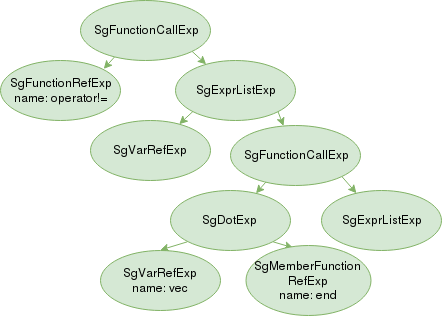
\includegraphics[height=6.2cm]{images/overloaded-cmp.png}
        \caption{Overloaded Not-Equals Comparison}
        \label{for-cmp-neq-overloaded}
    \end{subfigure}
  \hfill
  \begin{subfigure}[b]{0.4\textwidth}
        \centering
        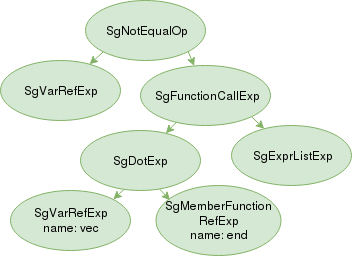
\includegraphics[height=4.5cm]{images/non-overloaded-cmp.png}    
        \caption{Not-Equals Comparison}
        \label{fig:for-cmp-neq}
    \end{subfigure}
    
    \caption{Not-equals Operators}
    \label{fig:comp-operators}
\end{figure}


\subsection{Loop header checks}

The main traversal first checks if the loop is of iterator type, Figure \ref{fig:code-for-iter}, by checking the initialise statement, comparison expression and increment expression. If the Initialisation check, \texttt{ hasValidInitializer}, finds a valid initialiser with an object making a call to \texttt{begin()}, the function extracts the name of the object and variable being assigned, setting the container name and iterator name, respectively. The names of the container and the iterator are then used in the further checks of comparison and the iterator expressions. The check of the comparison expression, \texttt{hasValidComparitor}, required handling containers, e.g List, Vector, utilising overloaded operators, so both overloaded and non-overload not equals operators had to be checked, Figure \ref{fig:comp-operators}. The increment check also had to account for the overloading of the \texttt{++} operator on the iterator extracted from the initialise statement. 


% checks on loop headers 2 
The array-like container case and the statically allocated array case can share the same checks for a valid initialiser, \texttt{hasValidIndexInitialiser(..)}, and increment expression, \texttt{hasVaildIncrement}. The valid increment check can be the same check utilised by iterator for loop case as well as it handles overloaded and standard \texttt{++} operators. The shared check, \texttt{hasValidIndexInitialiser}, which ensures that the initial value of the indexing variable is 0 ,Figure \ref{fig:code-for-container},  does not restrict matching to standard integer zeros, it supports long integers, \texttt{0l, 0L}. The check also handles any implicit or explicit casting that can occur from the type utilised by the variable. The check returns false if the indexing variable is assigned any variation of a double value. This restriction is instated to simplify the process of extracting the value and comparing it to zero.


The differences between the array-like container and the statically allocated array centre around the comparison check. For the array like container the check \texttt{hasVaild SizeComparitor(..)} , checks the index is compared against the container calling end, \texttt{COND.end()}. The decision was made to only support direct uses of the container, references to them are rejected, so only the dot notation for method calls is checked. Unlike the iterator case, the container is not present in the initialise statement, the first time it is seen in the array-like case is in the comparison expression. So it is here that the container is extracted to be utilised later in identifying the container in the loop body.

\subsubsection{Locating the Array being indexed}

The statically allocated array case required a unique approach to the comparison check, \texttt{hasVaildBasicComparator(..)}, as the index is compared to the size of the array before we have a reference to the container which is the focus of the for loop, Figure \ref{fig:code-for-stat}. To be able to check that the index is bounded by the size of the array, the array has to be known. So the hasVaildBasicComparator function utilises a new traversal class ValidArrayIndexTraversal to scan the loop's body to locate the container that is being indexed. The traversal does not aim to assess the safety of the transformation on the loop body, as this would overcomplicate the traversal. Not assessing the safety in ValidArrayIndexTraversal also increases reusability as same loop safety check traversal, \texttt{safeIndexForTransform(..)}, can be used by the statically allocated array and the array-like cases. 

\begin{figure}[H]
    \begin{subfigure}[b]{0.6\textwidth}
        \centering
        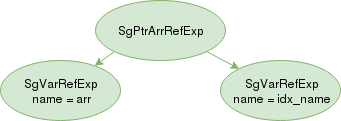
\includegraphics[width=0.8\textwidth]{images/ArrPtrAcc.png}
        \caption{AST of the function}
        \label{fig:arr-acc-AST}
    \end{subfigure}
    \hfill
    \begin{subfigure}[b]{0.4\textwidth}
        \centering
        \begin{minted}{C++}
            ...
        arr[idx_name]
            ...
        \end{minted}
        \caption{Code the AST is representing}
        \label{fig:arr-acc-code}
    \end{subfigure}
    \vspace{-0.5cm}
    \caption{Array access notation}
    \label{fig:arr-access}
\end{figure}

The \texttt{ValidArrayIndexTraversal} traversal searches for all pointer array reference expressions nodes, Figure \ref{fig:arr-access}, in the loop body then checks that the right hand side node is a variable reference to the index variable, \texttt{idx\_name}. If the index does match the variable declared in init-expression of the for loop, and the left-hand side of the array access is a variable reference, the array the variable refers to it set as the focus of the for-loop. Upon finding a suitable array, and before continuing the traversal, the size of the statically defined array is extracted and stored in a field in the traversal object along with the arrays name. 

\begin{figure}[H]
    \begin{subfigure}[b]{0.5\textwidth}
        \centering
        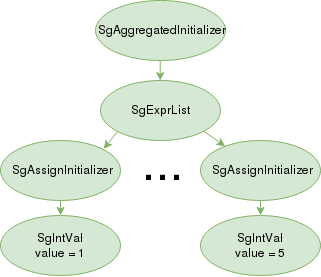
\includegraphics[height=5.6cm]{images/init-list.png}
        \caption{List initialisation AST}
        \label{fig:list-init-AST-var}
    \end{subfigure}
    \hfill
    \begin{subfigure}[b]{0.5\textwidth}
        \centering
        \begin{minted}{C++}
    int arr[] = {1,2,3,4,5};
        \end{minted}
        \caption{List initialisation code}
        \label{fig:list-init-var-code}
    \end{subfigure}
    \vspace{-0.5cm}
    \caption{List initialisation of an Array}
    \label{fig:list-init-var}
\end{figure}

The size of the array is found by examining the declaration of the array, a pointer to it is stored in the SgVarRefExp node. The declaration can take the forms shown in Figure \ref{fig:code-static-for-cm} as well as a list initialisation. So  can be extracted from the non-list initialisation declaration by accessing the type of the variable declaration, SgArrayType, then getting size value with the function, \texttt{arraytype->get\_index()}. To uncover the size of the list initialised array, the number of child nodes of the \texttt{SgExprListExp} needed to be retrieved, Figure \ref{fig:list-init}. 

After the container name and size have been extracted, the traversal continues searching all SgPtrArrRefExp, node and if another array with a different name meets the matching criteria the traversal set its \texttt{valid} field to false. So the \textit{hasVaildBasicComparitor} can check this field and return false once the traversal of the body end, stopping the transformation of that for-loop. If only a single array is found the validation of the comparison expression proceeds similarly to the array-like container check, ensuring that the value used in the comparison matches the actual array size from the traversal.  

\subsection{Safe to transform checks}

After the loop has matched to a supported loop type with the loop components being validated, the loop body needs to be confirmed safe to transform before proceeding. It was decided that to simplify the code and the transform's design, two separate traversals of the loop body would be utilised, one traversal for iterator loop type, \texttt{IteratorUseTraversal}, and another for array-like and statically allocated loop types, \texttt{IndexUseTraversal}. 

The \texttt{IteratorUseTraversal} searches for every SgVarRefExp nodes seeing if the variable name matches either the name of the iterator variable or the container, handling them separately. As the transform is interested in where the variables are being used, the parent node of the SgVarRefExp node is extracted, \texttt{varRef->get\_parent()}. The only acceptable parent nodes for the iterator variable are SgPointerDerefExp for non-overloaded dereference, SgArrowExp for non-overloaded access to methods using arrow expression, and finally, SgDotExp nodes which represent function calls on the iterator as it is an object. As the SgDotExp node has the iterator name on the left-hand side of the operation the only allowed methods to be called are \textit{operator*} and \textit{operator$\rightarrow$} representing the overloaded versions of the previously mentions expression. The reasons for only accepting these nodes and overloaded operators were discussed in Section \ref{sec:safety-of-trans}. If a container variable is found in the loop's body, independent and is not a child of one of the mentioned parent nodes, the loop body is marked as unsafe to transform.

The \texttt{IndexUseTraversal} traversal similarly checks every SgVarRefExp node and extracts the parent node if the variable name matches the container or index. As this traversal handles both array-like and statically allocated arrays it needs to handle the overloaded operator, \textit{operator[]} and the \texttt{at(..)} method call as well as normal array access notation represented by the SgPntrArrRefExp node in the AST. The index's allowed parent nodes are SgExprListExp which represents the arguments to a function call and the previously mentioned SgPntrArrRefExp node for non-overload access. To check that the function call is to only the allowed operators, the parent of the argument list needs to be check, as it is the root of the function call, SgFunctionCallExp.

% image of a function call  

\subsection{Building Ranged-for statement}\label{sec:build-range-for}
After the loop body has been confirmed to be safe the transformation of the for-loop can begin. To start with the transform creates a new ranged-for statement to replace the existing for statement. The function \textit{constructRangedBasedForLoop(..)} was created to build the ranged-for node, SgRangeBasedForStatement, requiring only the names of the container/array and the iterator/index. The function utilises the SageBuilder interface for constructing statements, the interface is used to build the variable declaration that will be the range-declaration, Figure \ref{fig:range-for-header-form}. The Figure \ref{fig:range-dec-var} shows the construction of the variable. The type is set to utilise \texttt{auto} type inference, as the extraction of type information from containers such as \texttt{vector<int>} is overly cumbersome as the template instantiated code in the AST does not make it simple. 

The final step in creating the range-based for are shown in Figure \ref{fig:range-based-for-stmt}. Many of the arguments for the build function can be omitted as we are not required to compile the code from the AST, as we unparse the AST to source-code. The only required statements are the range\_variable previously build and a declaration matching that of the container/array utilised called range\_var. The loop body is left empty as it will be replaced by the transformed loop body of the original for-loop.

\begin{figure}[H]
    \centering
    \begin{minted}{C++}
    SgVariableDeclaration* range_variable =
        buildVariableDeclaration(iterName, 
            buildReferenceType(
                buildTemplateType("auto"))); 
    \end{minted}
    \caption{Building range-declaration variable}
    \label{fig:range-dec-var}
\end{figure}

\begin{figure}[H]
    \centering
    \begin{minted}{C++}
SgRangeBasedForStatement* rangeFor =
    buildRangeBasedForStatement_nfi(range_variable,
                                    range_var,
                                    NULL, NULL, NULL, NULL,
                                    buildBasicBlock());    
    \end{minted}
    \caption{Building Ranged-based For}
    \label{fig:range-based-for-stmt}
\end{figure}

\subsection{Transformation of loop body}

The transformation of the loop body is achieved by yet another traversal through the loop body. Two separate traversals exist, \texttt{IteratorUseTransform} for the iterator case, and \texttt{IndexUseTransform} for array-like and statically allocated cases. The decision to create a separate traversal for checking the safety of the loop body and transforming it was to simplify the traversal and to not prescribe too much functionality to a single traversal. If a single traversal was utilised it would require implementing a form of backtracking to undo changes when traversing the loop body or to copy the loop body's AST. Depending on the size of the loop body this could greatly impact performance and memory use. As the backtracking approach would increase the complexity of the traversals the two traversal approach was taken.

\begin{figure}[H]
    \begin{subfigure}[b]{0.5\textwidth}
        \centering
            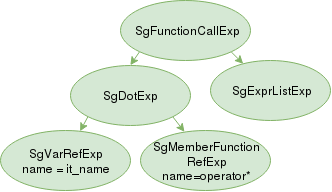
\includegraphics[height=4.1cm]{images/iterator-deref-replace-ast.png}
        \caption{AST of iterator dereference}
        \label{fig:iter-AST-Trans-deref-before}
    \end{subfigure}
    \hfill
    \begin{subfigure}[b]{0.5\textwidth}
        \centering
            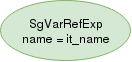
\includegraphics[width=0.42\textwidth]{images/single-varRef-node.png}
        \caption{After transform of iterator dereference}
        \label{fig:iter-AST-Trans-deref-after}
    \end{subfigure}
    \vspace{-0.5cm}
    \caption{Transformation of Iterator dereference}
    \label{fig:iter-deref-use-trans}
\end{figure}

The \texttt{IteratorUseTransform} traversal searches the loop body for all variable use nodes, SgVarRefExp, where the variable name matches the iterator name. Similarly to the safety traversal the parent node of the SgVarRefExp node is extracted and checked the node is of a certain type, e.g SgDotExp, SgArrowExp or SgPointerDerefExp. As most iterators overload there uses of $\rightarrow$, and $*$, the following discussion will focus on those cases, the non-overloaded cases are also handled in the traversal due to containers like \texttt{std::array} which do not overload them. If the parent node is a SgDotExp then a function call is present and from the safety check, we can assume it is either calling \textit{operator*} or \textit{operator$\rightarrow$}. Figure \ref{fig:iter-deref-use-trans} shows the transformation that takes place when the call is to \textit{operator*}. The AST need to be traversed upwards until the root of the function call expression, SgFunctionCallExp, is reached where it along with it's sub-tree is replaced by the SgVarRefExp node of the range-declaration statement, \texttt{it\_name}, Figure \ref{fig:iter-AST-Trans-deref-after}. 

\begin{figure}[H]
    \begin{subfigure}[b]{0.5\textwidth}
        \centering
            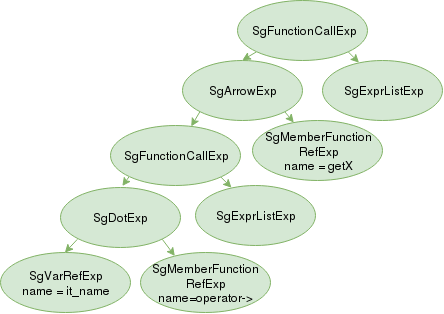
\includegraphics[height=5.5cm]{images/iterator-arrow-replace-ast.png}
        \caption{AST of iterator arrow expression}
        \label{fig:iter-AST-Trans-arrow-before}
    \end{subfigure}
    \hfill
    \begin{subfigure}[b]{0.5\textwidth}
        \centering
            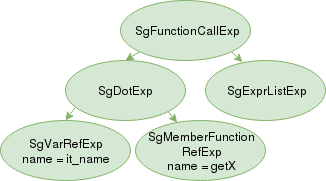
\includegraphics[width=0.8\textwidth]{images/iterator-arrow-replace-ast-after.png}
        \caption{After transform of iterator arrow expression}
        \label{fig:iter-AST-Trans-arrow-after}
    \end{subfigure}
    \vspace{-0.5cm}
    \caption{Transformation of overloaded iterator arrow expression}
    \label{fig:iter-arrow-use-trans}
\end{figure}

If the function call expression is to \textit{operator$\rightarrow$} then a more complex replacement is required as it features an associated function call after the arrow notation, Figure \ref{fig:iter-arrow-use-trans}. After the loop header has been altered the elements can be directly accessed, so the arrow expression has to be replaced by the dot expression, Figure \ref{fig:iter-AST-Trans-arrow-after}. 

The traversal \texttt{IndexUseTransform} for array-like and statically allocated cases, follows a similar process to the \texttt{IteratorUseTransform} traversal. The focus of this traversal is on transforming the code shown in Figure \ref{fig:before-tran-idx}, the traversal searches the loop body for all instances of variable use nodes names that match the array/container specified in the loop header checks. The transform then checks that the index is the only argument to the overloaded, \texttt{operator[]}, the \texttt{at(..)} or non-overloaded \texttt{[]} for statically allocated array. Upon passing the final check the entire array access expression  is replaced using the function \texttt{replaceExpressionCheck(arrAccess, buildVarRefExp(idx\_name)} provided by SageInterface.

The final stage of the transformation, after transforming the loop body, is to assembly the range-for node that will replace the for loop node, SgForStatement. Figure \ref{fig:replacing-for-loop-node} shows the process of the replacement, from the creation of the ranged-for node to the setting of its loop body to the transformed body of the original for-loop. After this process has completed the transformation exits and the newly transformed AST is passed to the Rose framework backend to be un-parsed back into source-code.
% add AST before and after images would be the most useful mirrors the 

\begin{figure}[H]
    \centering
    \begin{minted}{C++}
SgRangeBasedForStatement*rangeFor =
constructRangedBasedForLoop(containerName, iteratorName, loopNode);

IndexUseTransform indexUseTransform(containerName, iteratorName);
indexUseTransform.traverse(loopBody, preorder);

rangeFor->set_loop_body(loopBody);
replaceStatement(loopNode, rangeFor);
    \end{minted}
    \caption{Process of replacing the loop body}
    \label{fig:replacing-for-loop-node}
\end{figure}

% Over arcing structure
    %  main traversal
        %  compiler generated check
    %  checks on loop headers
        % indexing cases needing checking on zero values and casting ? 
    %  safe to transform traversals, different for iter and other 2 cases
        % overloading operators problems difference between container and static array
        % same traversal for statically allocated and array-like container 
        % differ
    %  generating new loop ranged-for header 
        % why use auto, extracting type is hard
    %  actual transformation pass over the loop body 
        %  why it can't be a single pass, easier than a back tracking approach
        %  how replacement works, search for each use of index unsure that its parent node is the array access expression with the array being the container 
%  extra: casting issues

\section{Evaluation}
The for-loop-rejuvenation defined in the previous sections will be evaluated, in a similar manner to auto-rejuvenation tool with a comparison to an existing clang-tidy tool. The evaluation will compare what the transforms target, how they assess the safety of transformation and their response to running on real-world programmes.   

\subsection{Testing of rejuvenation and comparison to clang-tidy}
As previous mentioned in Section \ref{sec:cmp-auto-reju-mod-auto} and related work Section \ref{sec:rw-clang-tidy}, clang-tidy features a set of modernize checks. The most relevant for comparing to the for-loop-rejuvenation is the the modernize-convert-loop \cite{FOR_CONVERT}, previously mention in Section \ref{sec:rw-clang-tidy}. As the for loop types targeted by for-loop-rejuvenation, Section \ref{sec:forLoop-scope-trans}, were based on those defined by the modernize-loop-convert check, the comparison between the tools is made easier. Both transformations handle loops over statically allocated arrays, containers using iterators and array-like containers using \texttt{at()} or \texttt{[]}. The transforms differ though in how they assess the safety of a transformation and how open or restrictive they are in allowing for-loops into each category. 

The modernize-loop-convert implements a set of confidence levels, risky, reasonable and safe, which dictate if the loop body is safe enough to allow for the transformation of the loop. The risky confidence setting allows for loops to be transformed where methods of the container are called in the loop body, reasonable confidence allows the conversion of those containers which make calls to new \texttt{end()} or \texttt{size()}, similarly to the case shown in Figure \ref{fig:code-for-container}. Finally, the safe confidence level allows only the for loops that do not have criteria that would place them in the other two levels.

The testing of for-loop-rejuvenation and modernise-loop-convert was conducted on a set of real-world code sampled from existing SPEC 2017 CPU benchmarks. All the files utilised were designated pure C++ and were taken from 541.leela\_r \cite{SPEC_LEELA}, 5531.deepsjeng\_r \cite{SPEC_DEEPSJENG} and 523.xalancbmk\_r \cite{SPEC_XALANCBMK} benchmarks. The results from the testing are displayed in Table \ref{tab:for-tool-benchmark}. The columns denoting the number of converted for loops shows that both transforms have a low hit rate at transforming for-loops. This in no ways suggests the tools are defective or wrong as they are limited by the fact that most for loops do not fit the template of ranged-for loops, not without completely changing the intended purpose of the loop. However, the test data does show that the impact the for-loop-rejuvenation can have, in its current form, is limited as it may be too restrictive in selecting for loops for transformation.

A reason for the reduced transformation rate in the for-loop-rejuvenation can be found in inspecting the for loops in the files that are not being transformed. The file \textit{bitboard.cpp} in the \textit{deepsjeng} benchmark had a large number of for loop, 34, but a zero transformation rate, an example of one of its for loops is shown in Figure \ref{fig:code-untrans-example}. The example shows that it is impossible for the transformation to proceed as the loop does not have a single array as its focus but two. The \textit{bitboard} file faces this problem as nearly all its for-loops need to access multiple arrays of type \texttt{BITBOARD} to calculate results.

\begin{figure}[!ht]
    \centering
    \begin{minted}{C++}
            BITBOARD DiagMaska1h8[64],DiagMaska8h1[64];
            for (i = 0; i < 64; i++){
                DiagMaska1h8[i] = 0;
                DiagMaska8h1[i] = 0;
                        ...
            }
    \end{minted}
    \caption{Example of a transform that is impossible}
    \label{fig:code-untrans-example}
\end{figure}

The previous example showed the impracticality of the transformation in some cases, but this is not the only reason some for-loops are ignored. The file \textit{TraverseSchema} from \textit{xalancbmk} benchmark suffers from a similar situation of having many for loop and non being selected for transformation. Figure \ref{fig:no-rejuv-indirect-var} shows one of \textit{TraverseSchema}'s for loop header, that could actually be transform as the loop body has no conflicts and the loop is bounded by a call to the \texttt{size} method of \texttt{fIC\_Elements}. However, currently in for-loop-rejuvenation, this is rejected as the transform would not identify the loop header as array-like but statically array then error on not finding an integer value after analysing \texttt{icListSize}. This loop form could be handled if references to containers were excepted along with array-like loops also allowing variable in the comparison expression for size. The problem remains, how far should the transformation follow the expression to determine if a loop is transformable. In this case the call to \texttt{size} is only contained in a local variable \texttt{icListSize = fIC\_Elements->size()} but if the variable utilised was an argument that had been passed to the function the difficulty increases dramatically. 

\begin{figure}[H]
    \centering
    \begin{minted}{C++}
            unsigned int icListSize = fIC_Elements->size();
            for (unsigned int i=0; i < icListSize; i++){ 
                            ... 
            }
    \end{minted}
    \caption{Example of possible transformation missed}
    \label{fig:no-rejuv-indirect-var}
\end{figure}

% round off
The examples of for-loops displayed above show that there are common patterns to their use and that those patterns, that can be transformed, could be added to the transformation, but capturing all possible patterns would be unfeasible and lead to an explosion in complexity. The current effectiveness of the for-loop-rejuvenation tool is lacking as can be seen from Table \ref{tab:for-tool-benchmark} and the examples above. To increase the effectiveness in a meaningful way an analysis of the most utilised pattern of for-loop use could find the uses like those in Figure \ref{fig:no-rejuv-indirect-var} and integrate them into the rejuvenation to build a more effective tool.

\section{Summary}
This chapter introduced the for-loop-rejuvenation and explored the transforms set of rules for detecting for-loops and checking their safety. The transform aims to increase the readability and maintainability of for-loops by utilises the ranged-for loop construct introduced in C++11. Through testing and comparison to similar tools, it can be seen that the rejuvenation is limited in its effectiveness, as the number of possible loops to transforms is a subset of the total number of loops. The rejuvenation also suffers from an overly restrictive approach in selecting those remaining for-loops for transformation.

The for-loop-rejuvenation does show how a rejuvenation can handle spanning transformations, as the entire loop body needs to be traversed to ensure the for loop is valid for use with a range-for construct. The for-loop-rejuvenation however only traverses or makes changes with the scope of the for loop, more elaborate rejuvenations such as identifying and transforming user defined linked lists to\textit{ std::list}, which would require checks spanning entire files and identifying multiple functions and uses. This complex spanning rejuvenation shows that rejuvenation can target large scale structures which could greatly increase the maintainability of old code by offering a standard interface, \texttt{std::list}, after the transformation.


% does have its benefits, readability

% results transform limited in its effect, ranged-for loops are only useful or usable in a very limited setting

% the span of the transformation restricted to the body of the for loop, other rejuvenation can go further than that 

% more elaborate experiments detecting user defined linked lists 


\begin{landscape}
\begin{table}[H]
\centering
\begin{tabular}{|l|l|l|l|l|l|}
\hline
Benchmark Test & File Name & \# of Lines & \# of for loops found & \# of trans rose-tool & \# of trans clang-tidy \\ \hline
541.leela\_r & FastBoard.cpp & 2452 & 85 & 3 & 2 \\ \hline
 & GTP.cpp & 502 & 6 & 1 & 1 \\ \hline
 & FastState.cpp & 479 & 21 & 0 & 0 \\ \hline
 & UCTSearch.cpp & 469 & 0 & 0 & 0 \\ \hline
 & UCTNode.cpp & 456 & 3 & 0 & 0 \\ \hline
 & Matcher.cpp & 100 & 3 & 0 & 0 \\ \hline
 & SGFTree.cpp & 357 & 7 & 0 & 0 \\ \hline
531.deepsjeng\_r & search.cpp & 1936 & 17 & 0 & 2 \\ \hline
 & utils.cpp & 1109 & 16 & 0 & 0 \\ \hline
 & pawn.cpp & 761 & 1 & 0 & 0 \\ \hline
 & bitboard.cpp & 547 & 34 & 0 & 0 \\ \hline
 & epd.cpp & 477 & 3 & 0 & 0 \\ \hline
 & ttable.cpp & 278 & 5 & 0 & 0 \\ \hline
 & moves.cpp & 227 & 18 & 0 & 0 \\ \hline
523.xalancbmk\_r & TraverseSchema.cpp & 9060 & 39 & 0 & 0 \\ \hline
 & SGXMLScanner.cpp & 4752 & 10 & 0 & 0 \\ \hline
 & IGXMLScanner.cpp & 3296 & 5 & 0 & 0 \\ \hline
 & DGXMLScanner.cpp & 3245 & 4 & 0 & 0 \\ \hline
 & IGXMLScanner2.cpp & 3240 & 8 & 0 & 0 \\ \hline
 & XMLUri.cpp & 2569 & 6 & 0 & 0 \\ \hline
 & XTemplateSerializer.cpp & 2383 & 43 & 0 & 0 \\ \hline
 & SchemaValidator.cpp & 2195 & 16 & 0 & 0 \\ \hline
 & WFXMLScanner.cpp & 2150 & 5 & 0 & 0 \\ \hline
\end{tabular}
\caption{Benchmark Test data of for loop transforms }
\label{tab:for-tool-benchmark}
\end{table}
\end{landscape}

% Comparison to clang-tidy modernise-for-loop + Testing
    % explain what modernise-loop-convert does 
        % target transformation similar to the designed tool risky setting adjusted
        % risky settings
        % handles types in for loop more sensible - not always using auto
    % showing table of data from benchmarks
        % number of hits on benchmarks
        % oracle to see how good performance is
        % what can be drawn from this comparison 

% Limitations of the transformation
    % cases where it can be used are limitied 
    % can't catch most use cases of passing a variable to the statically allocated 
    %   array as variable is passed through a function.

% possible extensions - some what interesting
    % smarter types extraction for loop instead of always utilising auto

\chapter{Conclusion \& Further work}
% intro, what this chapter will contain 
The following chapter provides a conclusion to the report, summarising the evaluations of the source code rejuvenations as well as presenting an explanation of the wider problems faced in designing source code rejuvenation tools. A discussion of further work is also included referencing again the simple extensions than can be made to the source code rejuvenations presented in the report. After the possible changes to the current tools are show, additional passes which could offer rejuvenations to other areas of source code are presented. Finally, a discussion of a different approach to designing source code rejuvenations is given, focusing on how a new approach can help simplify the creation of new tools.   

\section{Conclusion}
% summary of results explainations of what was found/discovered when designing and evaluating the tools
\subsection{Discuss of auto-rejuvenation}

The first Source code rejuvenation featured in the report, \textit{auto-rejuvenation}, suffered several conceptual problems in its approach to performing its rejuvenation of variable declarations. A central problem identified when transforming variable declarations type signatures, to utilises the \texttt{auto} keyword, was that in many places replacing the type lead to harder to read code as information provided in the type which add context to the declaration was being removed, Figure~\ref{fig:reduce-info-auto}. 

\begin{figure}[H]
    \centering
    % \includegraphics{}
    \caption{Example: utilising \texttt{auto} reduces contextual information for variable}
    \label{fig:reduce-info-auto}
\end{figure}

Another problem from the over application of the \texttt{auto} keyword was that basic types did not gain anything from utilising \texttt{auto} as types such as \texttt{int}, \texttt{bool} and \texttt{char} all are of equal length to \texttt{auto}. So replacement is seen as meaningless in the best scenario or hurtful if it reduces useful context to the programmer. The meaningless or hurtful replacements of certain type signature introduced an important consideration when designing rejuvenation, in that applying new features to old code blindly does not amount to rejuvenation in the sense of improving code. Rejuvenation should be applied in ways to actually improve code so to bring new life to it by making it easier to maintain and extend. 

The problems related to the over application of \textit{auto-rejuveantions}'s transform showed the complexity of designing effective transforms and how careful thought is required when selecting the code to be transformed. As C++ is not a dynamically typed language so requires statically defined types these types become a part of the style of writing C++, so to aimlessly apply the transform is not advised. The use of \texttt{auto} does offer benefit of remove the verbose type signatures but a balance is required to produce the best possible outcome from transformation. (coding style plays a factor).

\subsection{Discussion of for-loop-rejuvenation}

The \texttt{for-loop-rejuvenation} suffers from distinct problems from the previous transformations as its hit rate, even on a large sample set, is near zero. The first factor attributing to this reduction was that many of the main patterns of using for-loops were not captured by the rejuvenation tool. Further reducing the hit rate is that many of the for-loops were impossible to transform to utilise the ranged-for construct as they do not feature a single array being completely traversed. Even those the second of the two factors would be impossible to solve, the first factor does allow for some solutions to improve the hit rate, such as identifying the most utilised patterns of for-loops in real-world code and augment the code to transform them. The identification of the most common ways old features or idioms are used is an importance technique which can be applied to a number of rejuvenations to increase the effectiveness.

The two previously mentions factors reducing the number of overall transformations are not specific to \textit{for-loop-rejuvenation}, as impossible transformations and missed opportunities could effect a wide range of rejuvenation attempts. These factors are central to designing rejuvenations and bring to light a number of trade-offs present when creating them, such as the complexity of the rejuvenation tool and its relation to the whether the target appears in real-world code. If a pattern in the AST is complex to match against and it does not appear in actual code then the usefulness of the rejuvenation is diminished and computation time and development time in designing the transform is wasted. 

% changing code and ensuring it actual makes improvements requires measuring of readability and maintainability

\subsection{Closing remarks}
There are many pitfalls and misguided improvements that can occur when developing rejuvenations so work needs to be done to ensure that rejuvenation actually improves the final code, and important areas for transformations are not missed. It is also critical to check that the suggested benefits to the code like maintainability and readability are actually being realised. This requires to be able to assess, with tangible metrics, the code before the transformation and after to be able to see improvements and so refrain from judging these aspects by developer intuition as this could boil down to personal preference. It is also clear from the source code rejuvenation seen in this report that in developing rejuvenations tools it is hard to balance the application of a transformation in terms of complexity and scope with the effective results, readability and maintainablity, on the final source code produced. 

% conclude with this statement
% the transforms given above show how hard it can be to balance complexity with the scope and effectiveness of transformations  

\section{Further work}
% more complex rejuvenation pass with requires several passes over the source code or require large spanning checks on the ast, like detecting user defined linked lists 
% extension for the for-loop-reju addition pre traversal pass to allow for better 

\subsection{Extensions to current souce code rejuvenations}
In the evaluation of the source code rejuvenations additional extensions where given for both the \textit{auto-rejuvenation} and  \textit{for-loop-rejuvenation}. It was suggested that the \textit{auto-rejuvenation} which was previously restricted to using \texttt{auto} on variable declarations also be allowed to utilise \texttt{auto} for the return type of the function declarations, Figure \ref{fig:funct-ret-inferred}.

The suggested extension to \textit{for-loop-rejuvenation} was the additional use of a wider range of patterns more inline with the programmers actual uses of for-loops so to improve the rate at which they would be transformed to use the ranged-for construct.

% The \textit{for-loop-rejuvenation} suggested extension was to add additional an additional traversal pass to allow for constant propagation through the use of function to allow for the case where the for-loop takes place inside a function where the size of the array being iterated over is taken as an argument, Figure \ref{}. This was previously not possible as for statically allocated arrays is would try to follow the variable utilising the slide  

%  additional utilisation become available for the keywords between uses 

\subsection{Additional source code rejuvenations}
The number of possible rejuvenations even within the C++ language is much larger than the those discussed in this report. A further rejuvenation which could be implemented is the detection of user defined linked lists and transform there use to utilise a standard library implementation such as \texttt{std::list}. The complexity of this source code rejuvenations lays in two areas, identifying an occurrence of a user defined list and detecting the type of list it is. Identifying a user defined linked list is more complicated than both of the rejuvenation tools discussed previously as the implementation of the list could be spread throughout the source file, and requires checking the definitions and several functions to see if the operations defined for the list are in line with those also provided by different standard library list implementations. As the ways to implement a list are very open ended the transform would have to handle a very wide scope of definitions for a list as well as differentiating between doubly linked list, circular list and singly linked lists.

% example
\begin{figure}[H]
    \centering

    \caption{Example of a user defined list in C}
    \label{fig:user-def-list}
\end{figure}

The transformation process for the uses of a user defined lists also introduces new challenges as the definition of the list could be in a different file from where it is being used. So the definition of the user defined list is required to be known before traversing the source code file or files of the project to transform the instances where it is utilised, which will require an initial traversal through the project to know of its existence. Also when an instance of a variable using the user defined list can be replaced with standard library implementation then all further use of the list also needs to be transform to utilise the functions defined for the standard library's interface. This type of traversal is even more spanning than the localised case of the for-loop-rejuvenation which was restricted to loop body.

The benefits of rejuvenating user defined lists are the well documented interfaces to the standard library implementations which means that developer will not have to search for and try to understand the those implement in the old code which could lack useful documentation. The standard library implementations also offer tried and tested implementations which are significantly less likely to include bugs than those found in unmaintained code.

\subsection{Developing future rejuvenations}
One of the main difficulties of implementing source code rejuvenation in frameworks like the Rose compiler is the verbose way required to match against segments of the AST. As can be seen in the implementation sections of source code rejuvenations produced in this report, searching for matching AST subtree requires checking each node for the correct type, requiring \texttt{NULL} checks and calls to subsequent child nodes. When using this approach, altering the code to allow for a more variation in matching of the AST (e.g matching multiple types of variable declarations) results in a large amount of additional type of node checks as well as complex conditional if logic. 

There is a desire to remove this requirement in having to detect target AST subtrees by matching individual nodes directly as it is more of an implementation detail than directly connected to the rejuvenation which is trying to be implemented. There has been additional to make the matching of AST subtrees or even individual nodes easier, clangs AST matchers \cite{} and Rose AST query interface \cite{}, but neither are directly focused at aiding source code rejuvenation. 

A solution to the problem could utilise a system similar to regular expressions for matching text \cite{} but with the of matching AST nodes as shown in the Figure \ref{fig:adv-ast-matching}. The the textual representation could utilise variable which are match in the underlying implementation, so for example the text used in Figure \ref{fig:adv-ast-matching} matches against all for-loops which have the same variable across all component which is labled as \$i. The implementation could handle other such 

 \begin{figure}[H]
    \centering
    \begin{minted}{C++}
    vector<SgNodes> rootNodesOfPattern =
        MatchPattern(astRoot,
            "for(int \$(i) = 0; \$(i) < \$NUMBER; \$(i)++")
    \end{minted}
    \caption{Possible textual representation of matching AST segment}
    \label{fig:adv-ast-matching}
\end{figure}



% simple extensions
    % reference the chapters and explain
% additional passes 
    % user defined linked list
        %  why it is hard
        %  how it can be more beneficial than previous passes
% creating a better interface to create transformations 
    % pattern matching interface 
    % 
    
% what am I actually going to build upon

% %%%%%%%%%%%%FORGOTTEN CHAPTERS%%%%%%%%%%%%%%%%%%%
% \chapter{Initialised List}
% \chapter{User defined Link List}
% \chapter{Results}
%%%%%%%%%%%%%%%%%%%%%%%%%%%%%%%%%%%%%%%%%%%%%%%%%%%

% use the following and \cite{} as above if you use BibTeX
% otherwise generate bibtem entries
\bibliographystyle{unsrt}
\bibliography{mybibfile}

\end{document}
